\documentclass[12pt,a4paper]{article}

\usepackage[utf8]{inputenc}
\usepackage[T1]{fontenc}
\usepackage[brazil]{babel}
\usepackage{mathptmx}
\usepackage{amsmath,amssymb}
\usepackage[a4paper,margin=2.5cm,headheight=14.5pt]{geometry}
\usepackage{setspace}
\usepackage{indentfirst}
\usepackage{microtype}
\usepackage{graphicx}
\usepackage{booktabs}
\usepackage{array}
\usepackage{caption}
\usepackage{float}
\usepackage{enumitem}
\usepackage{tikz}
\usepackage{newfloat}
\usepackage{fancyvrb}
\usepackage{fvextra}
\usepackage{fancyhdr}
\usepackage[hyphens]{url}
\usepackage[round,semicolon,authoryear]{natbib}
\usepackage[hidelinks]{hyperref}

\onehalfspacing
\frenchspacing
\setlength{\parindent}{1.25cm}
\setlength{\parskip}{0pt}
\raggedbottom
\setlist{itemsep=0.25em,topsep=0.4em}
\captionsetup{font=small,labelfont=bf,skip=6pt}
\DeclareFloatingEnvironment[fileext=loa,listname={Lista de algoritmos},name=Algoritmo,placement=htbp]{algoritmo}
\graphicspath{{figuras/}}
\urlstyle{rm}

\pagestyle{fancy}
\fancyhf{}
\fancyhead[R]{\thepage}
\renewcommand{\headrulewidth}{0pt}
\fancypagestyle{plain}{%
  \fancyhf{}%
  \fancyhead[R]{\thepage}%
  \renewcommand{\headrulewidth}{0pt}%
}
\numberwithin{equation}{section}

\makeatletter
\renewcommand{\@biblabel}[1]{}
\makeatother
\setlength{\bibhang}{1.25cm}

\title{História do Cálculo Numérico e sua Relação com a Ciência da Computação: Estudo e Implementação dos Métodos de Runge-Kutta na Simulação de Circuitos RLC}
\author{Jonathan Drumond}
\date{2026}

\begin{document}

\begin{titlepage}
\hypersetup{pageanchor=false}
\thispagestyle{empty}
\centering
{\large INSTITUTO FEDERAL DE EDUCAÇÃO, CIÊNCIA E TECNOLOGIA DO CEARÁ\par}
\vspace{0.35cm}
{\large Departamento de Telemática\par}
\vspace{0.25cm}
{\large Curso de Engenharia de Computação e Engenharia de Telecomunicações\par}
\vspace{1.8cm}
{\large\bfseries Cálculo Numérico\par}
\vspace{1.6cm}
{\Large\bfseries História do Cálculo Numérico e sua Relação com a Ciência da Computação: Estudo e Implementação dos Métodos de Runge-Kutta na Simulação de Circuitos RLC\par}
\vspace{2.2cm}
{\large Jonathan Drumond\par}
\vspace{1.6cm}
{\large Prof.\ Dr.\ Francisco J.\ A.\ de Aquino\par}
\vfill
{\large Fortaleza -- CE\par}
\vspace{0.2cm}
{\large 2026\par}
\end{titlepage}
\hypersetup{pageanchor=true}

\pagenumbering{arabic}
\setcounter{page}{1}

\section*{Resumo}
\addcontentsline{toc}{section}{Resumo}

Este trabalho articula a história do cálculo numérico com a ciência da computação e aprofunda os métodos de passo único para equações diferenciais ordinárias. O problema de engenharia é o circuito RLC série, tratado como protótipo de um estágio ressonante de comunicações. O modelo de estados, nas variáveis corrente e tensão no capacitor, é integrado pelos métodos de Euler, de Euler melhorado e de Runge-Kutta clássico de quarta ordem, implementados em Python sem integrador de biblioteca. As soluções numéricas são comparadas às formas fechadas do degrau, nos regimes subamortecido, crítico e sobreamortecido, e da excitação senoidal dentro e fora da ressonância. O estudo varia o passo, o fator de qualidade, a precisão de ponto flutuante e a tolerância de um controlador adaptativo por duplicação de passo. No circuito com fator de qualidade igual a 5, as ordens observadas tendem a 1, 2 e 4. O limite de estabilidade do método de Euler coincide com o produto da resistência pela capacitância: 20~\(\mu\)s quando o fator de qualidade vale 5 e 2~\(\mu\)s quando vale 50. O Runge-Kutta de quarta ordem permanece estável até cerca de 285~\(\mu\)s nesse segundo caso. Em precisão simples, o erro deixa de cair com o refinamento do passo e estaciona na casa de \(10^{-8}\)~A; em precisão dupla, o mesmo método chega à casa de \(10^{-16}\)~A. A ordem reduz o custo de uma precisão prescrita, e a região de estabilidade absoluta decide se a simulação de um tanque seletivo permanece física.

\vspace{0.6em}
\noindent\textbf{Palavras-chave:} cálculo numérico; método de Runge-Kutta; circuito RLC; estabilidade numérica; telecomunicações.

\clearpage
\tableofcontents
\clearpage

\section{Introdução}

Boa parte dos modelos usados em engenharia nasce contínua: tensões, correntes, campos e envelopes de sinais são descritos por equações diferenciais. O computador, por sua vez, só executa um número finito de operações aritméticas sobre quantidades representadas com precisão finita. O cálculo numérico é a disciplina que torna esse encontro rigoroso. Ele não substitui a modelagem; ele diz em que condições uma sequência discreta de operações produz uma aproximação confiável do modelo, quanto isso custa e quando o resultado deixa de ter sentido físico.

A história dessa disciplina é mais antiga do que a do computador eletrônico. Tabelas, logaritmos, interpolação e os primeiros métodos para equações diferenciais foram criados para o cálculo manual e para a produção de tábuas matemáticas. As máquinas de Pascal, de Leibniz e de Babbage, e depois os computadores programáveis do século XX, automatizaram procedimentos que a análise numérica já havia formulado. Compreender essa trajetória evita tratar o algoritmo como uma caixa atual, desligada das limitações de arredondamento, de estabilidade e de custo que o produziram.

O tema específico deste trabalho é a integração numérica de equações diferenciais ordinárias por métodos de passo único, com aprofundamento no método de Euler, no Euler melhorado e no Runge-Kutta clássico de quarta ordem. O problema de engenharia que conduz os experimentos é o circuito RLC série. Com uma escolha de parâmetros, o mesmo circuito descreve o transitório de um estágio ressonante: o tempo de acomodação de um filtro, o crescimento da corrente quando uma portadora entra em sintonia e o toque que um pulso curto deixa num tanque seletivo. Há solução analítica em vários casos, o que permite medir erro de verdade, e não apenas a diferença entre dois métodos.

O objetivo geral é elaborar um estudo que una a evolução histórica do cálculo numérico ao desenvolvimento da computação e que implemente, teste e critique um método numérico de interesse direto para a engenharia de computação e de telecomunicações. Os objetivos específicos são: situar o cálculo aproximado desde as tabelas até as bibliotecas científicas atuais; relacionar essa evolução aos instrumentos de cálculo e aos computadores eletrônicos; discutir ponto flutuante, erro, estabilidade e custo na implementação; aplicar os métodos a um circuito ressonante; e registrar, com código próprio, a convergência, a estabilidade e o efeito da precisão finita.

O texto está organizado da seguinte forma. A Seção~\ref{sec:historia} percorre a história pedida, das tábuas matemáticas à computação científica contemporânea. A Seção~\ref{sec:teoria} formula o problema de valor inicial, o modelo do circuito e a análise de erro e de estabilidade dos três métodos. A Seção~\ref{sec:algoritmos} descreve os algoritmos e a implementação. A Seção~\ref{sec:aplicacoes} liga o circuito às grandezas usadas em comunicações. A Seção~\ref{sec:resultados} discute os experimentos. A Seção~\ref{sec:conclusao} sintetiza os resultados e indica continuações. O código completo está no Apêndice~\ref{ap:codigo}.

\section{Referencial histórico}
\label{sec:historia}

\subsection{Tabelas, logaritmos e interpolação}

Durante séculos, calcular significou consultar e completar tabelas. Efemérides astronômicas, tábuas de tiro, tabelas de juros e funções transcendentes eram produzidas à mão, com conferência dupla, porque um dígito errado se propagava para todos os usuários da tábua. A interpolação era a ferramenta que extraía um valor intermediário sem refazer a conta inteira. As fórmulas de diferenças finitas, mais tarde associadas a Newton e a Lagrange, nasceram dessa oficina, não de uma preocupação abstrata com polinômios \citep{goldstine1972,burden2016}.

A invenção dos logaritmos, no início do século XVII, mudou o custo da multiplicação. Uma multiplicação virava soma de logaritmos, e uma raiz virava divisão do logaritmo. As tábuas de logaritmos passaram a ser infraestrutura de engenheiros, navegadores e astrônomos. A régua de cálculo é a versão analógica dessa ideia: escalas logarítmicas deslizantes fazem a soma dos logaritmos por um deslocamento mecânico. William Oughtred formulou a régua no século XVII, e o instrumento permaneceu na bancada de engenheiros até as calculadoras científicas eletrônicas da década de 1970 \citep{hopp1999,williams1997}. A precisão era de poucos algarismos, suficiente para uma estimativa de projeto e insuficiente para uma tabela fina. Essa limitação já anunciava um tema deste trabalho: o instrumento determina o erro tanto quanto a fórmula.

Havia também tabelas de números aleatórios. Antes de geradores computacionais confiáveis, simulação, estatística e criptografia usavam dígitos impressos. O caso mais conhecido é \emph{A Million Random Digits with 100,000 Normal Deviates}, publicado pela RAND Corporation em 1955, com um milhão de dígitos obtidos por um dispositivo eletrônico semelhante a uma roleta \citep{rand1955,lecuyer2017}. A curiosidade mostra o quanto o cálculo numérico dependia de objetos físicos, e não apenas de teoremas.

\subsection{De Newton a Runge e Kutta}

Isaac Newton deixou, no século XVII, o método das diferenças finitas e um procedimento iterativo para raízes de polinômios. Joseph Raphson publicou em 1690 uma forma mais direta desse procedimento, que a tradição posterior consolidou como método de Newton-Raphson, já com a derivada explícita. O uso imediato era corrigir tábuas e resolver equações que não se deixavam inverter em forma fechada \citep{burden2016,franco2006}.

Leonhard Euler publicou em 1768, no primeiro volume de \emph{Institutionum calculi integralis}, o que hoje chamamos de método de Euler para equações diferenciais: avançar a solução com a derivada do ponto atual multiplicada pelo passo \citep{euler1768,hairer1993}. A ideia é a definição de derivada lida ao contrário. Euler também desenvolveu a fórmula de Euler-Maclaurin, que liga somas a integrais e está na origem de várias correções de quadratura.

Joseph-Louis Lagrange reorganizou a interpolação polinomial e o cálculo de diferenças numa linguagem que ainda reconhecemos. Carl Friedrich Gauss, no começo do século XIX, deu forma sistemática à eliminação para os sistemas lineares dos mínimos quadrados da astronomia, e construiu a quadratura que leva seu nome. Um procedimento equivalente de eliminação já aparecia nos \emph{Nove capítulos da arte matemática}, na China antiga; o que Gauss fez foi torná-lo ferramenta regular da ciência aplicada \citep{goldstine1972,franco2006}. No século XIX, Carl Gustav Jacobi propôs um método iterativo para os sistemas lineares que surgem nos mínimos quadrados. A iteração de Jacobi, ao lado da de Gauss-Seidel, é o antepassado dos métodos usados hoje em sistemas esparsos de grande porte \citep{burden2016,ruggiero1996}.

A linha que este trabalho segue de perto começa no fim do século XIX. Carl Runge publicou em 1895 um método de integração que avaliava a função em estágios internos, em vez de exigir derivadas totais de ordem alta \citep{runge1895}. Karl Heun, em 1900, sistematizou a comparação com a série de Taylor e construiu métodos de ordem mais alta, entre eles o corretor que a disciplina chama de Euler melhorado \citep{heun1900}. Wilhelm Kutta, em 1901, deu a forma geral dos métodos explícitos de estágios e apresentou o método clássico de quarta ordem, com quatro avaliações da função por passo \citep{kutta1901}. Butcher e Wanner \citep{butcher1996} reconstruíram essa sequência e mostraram como as condições de ordem, a estabilidade linear e os métodos implícitos saíram dali no século seguinte. O algoritmo que um programa executa em poucas linhas foi, na origem, um substituto engenhoso da série de Taylor para quem calculava à mão.

\subsection{Instrumentos de cálculo}

O ábaco, em versões mesopotâmicas, romanas e chinesas, é o registro antigo de um princípio que a computação não abandonou: separar o estado (as contas) da regra (o movimento). A pascalina de Blaise Pascal, concebida em 1642, mecanizou a soma e o transporte. A calculadora de Gottfried Wilhelm Leibniz, o \emph{Stepped Reckoner}, estendeu a máquina às quatro operações por meio do cilindro dentado de Leibniz. No mesmo ambiente intelectual, Leibniz descreveu a aritmética binária em 1703 \citep{leibniz1703}. O texto é filosófico e matemático, não um projeto de computador, mas a representação que os circuitos digitais adotaram está formulada ali \citep{goldstine1972,williams1997}.

Charles Babbage deu o passo seguinte ao separar a produção de tabelas de um operador humano. A Máquina de Diferenças, projetada a partir de 1822, avaliava polinômios pelo método das diferenças finitas: depois de algumas colunas iniciais, só resta somar. A Máquina de Diferenças nº~2, desenhada entre 1847 e 1849, só foi construída pelo Science Museum de Londres na década de 1990, sob a coordenação de Doron Swade, e funcionou. O desenho de Babbage era viável; faltaram, no século XIX, dinheiro, tolerância mecânica e tempo político \citep{swade2001}.

A Máquina Analítica, descrita por Babbage a partir de 1837, já não era uma máquina de uma fórmula só. Tinha moinho (\emph{mill}), depósito (\emph{store}), cartões de operação e cartões de variável, inspirados no tear de Jacquard, e previa repetição e desvio. Não foi concluída. Ainda assim, é o primeiro projeto reconhecível de um computador de programa externo \citep{swade2001,goldstine1972}.

\subsection{Lovelace, Babbage e a ideia de programa}

Em 1843, Augusta Ada King, Condessa de Lovelace, traduziu para o inglês o artigo de Luigi Menabrea sobre a Máquina Analítica e acrescentou notas mais longas do que o próprio artigo \citep{menabrea1843}. A Nota G descreve, passo a passo, o cálculo dos números de Bernoulli na máquina. É o documento que a história da computação trata como o primeiro programa publicado. Lovelace também percebeu que a máquina manipulava símbolos segundo regras, e que o conteúdo desses símbolos não precisava ser apenas número no sentido aritmético estreito. A distinção entre o mecanismo e a sequência de operações é a distinção entre hardware e programa.

Babbage queria automatizar o cálculo que as tabelas exigiam. Lovelace descreveu a automação como uma linguagem de procedimentos. Os dois lados continuam no trabalho de quem implementa um método numérico: há a fórmula, e há a ordem das avaliações, os testes de parada e a representação dos dados. Sem essa segunda camada, o método de Kutta permanece uma receita de papel.

\subsection{Computadores eletrônicos e a arquitetura de von Neumann}

Entre a engrenagem e a válvula houve uma geração eletromecânica. O Z3 de Konrad Zuse, em 1941, operava com relés, aritmética binária de ponto flutuante e programa em fita perfurada. É amplamente reconhecido como o primeiro computador programável automático em funcionamento \citep{rojas1997}. O Harvard Mark I, de Howard Aiken, seguia a mesma família eletromecânica, em grande escala. Essas máquinas são a transição, não um detalhe: o cálculo deixou de ser um gesto da mão antes de deixar de ser mecânico.

O ENIAC, construído na Universidade da Pensilvânia por J. Presper Eckert e John Mauchly, com participação de Herman Goldstine, foi apresentado em 1946 para calcular tabelas balísticas. Era eletrônico, decimal, e a programação original era feita por cabos e chaves. Programar era reconfigurar o hardware. Em 1948 o ENIAC recebeu um modo rudimentar de programa armazenado \citep{goldstine1972}. Os cartões perfurados, herdeiros do sistema de Herman Hollerith para o censo americano de 1890, continuaram por décadas como suporte de programa e de dados. A separação entre escrever um algoritmo e executá-lo, hoje trivial, foi uma conquista material.

O texto que fixou a organização depois dominante é o \emph{First Draft of a Report on the EDVAC}, de John von Neumann, de 1945 \citep{vonneumann1945}. Unidade aritmética, memória que guarda instruções e dados, unidade de controle e órgãos de entrada e saída: a chamada arquitetura de von Neumann. O próprio Goldstine \citep{goldstine1972} registra que a ideia de programa armazenado foi elaborada no grupo da Moore School, com Eckert e Mauchly, e não por uma pessoa só. O primeiro programa armazenado executado numa máquina eletrônica correu no Manchester Baby, de Frederic Williams e Tom Kilburn, em 21 de junho de 1948. O EDSAC, de Maurice Wilkes, em Cambridge, entrou em serviço regular em 1949 e tornou o modelo utilizável para cálculo científico \citep{williams1997}. A partir daí, um método numérico podia ser texto, copiado e reexecutado, e não mais um painel de cabos.

\subsection{Aritmética binária, ponto flutuante e o limite do hardware}

O Z1 e o Z3 de Zuse já usavam ponto flutuante binário na passagem da década de 1930 para a de 1940 \citep{rojas1997}. A padronização que os computadores atuais seguem veio bem depois: o padrão IEEE 754, publicado em 1985 e revisado em 2008 e 2019, fixou formatos, arredondamentos e exceções \citep{ieee2019}. Um número em precisão dupla (\emph{binary64}) tem um bit de sinal, 11 de expoente e 52 de fração. A precisão simples (\emph{binary32}) tem 8 bits de expoente e 23 de fração. O épsilon de máquina, distância relativa entre 1 e o próximo representável, vale cerca de \(2{,}22\times 10^{-16}\) na precisão dupla e \(1{,}19\times 10^{-7}\) na precisão simples.

Essa representação não é um detalhe de implementação. Ela introduz erro de arredondamento em quase toda operação, faz somas deixarem de ser exatamente associativas e cria cancelamento quando se subtraem quantidades próximas \citep{goldberg1991,overton2001,higham2002}. Overflow, underflow e perda de dígitos significativos são limites físicos do formato, não falhas do método matemático. Numa integração longa, o erro de truncamento do método cai com o passo, enquanto o erro de arredondamento tende a crescer, porque há mais operações. A Seção~\ref{sec:precisao} mede esse cruzamento no circuito RLC.

O hardware também limita a estabilidade por outro caminho. Um método explícito exige um passo pequeno quando a dinâmica é rápida. Quanto maior a frequência do circuito, menor o passo em tempo absoluto para percorrer o mesmo número de períodos. O algoritmo pode ser o mesmo; o tempo de máquina não é.

\subsection{Linguagens e bibliotecas numéricas}

Enquanto o programa era escrito em código de máquina, o método numérico e o endereço dos registradores se misturavam. Fortran, desenvolvido na IBM por uma equipe liderada por John Backus, separou as duas coisas. O primeiro compilador foi entregue em 1957 para o IBM 704. A linguagem foi desenhada para traduzir fórmulas para código eficiente, e tornou-se o veículo do cálculo científico durante décadas \citep{backus1979}.

As bibliotecas seguiram essa vocação. Os Basic Linear Algebra Subprograms (BLAS), de 1979, padronizaram as operações de vetor e, nas extensões posteriores, de matriz \citep{lawson1979}. O LAPACK, a partir de 1992, construiu sobre o BLAS os métodos de álgebra linear densa usados por quase todo software científico \citep{anderson1999}. A FFTW mostrou que uma transformada tão clássica quanto a de Fourier ainda ganhava desempenho com planejamento automático e atenção à hierarquia de memória \citep{frigo2005}. O cálculo numérico de alto desempenho, hoje, é tanto matemática quanto organização de dados.

MATLAB nasceu no fim da década de 1970, quando Cleve Moler quis uma interface interativa para as bibliotecas LINPACK e EISPACK no ensino. A MathWorks foi fundada em 1984, e o programa tornou-se o ambiente padrão de muita engenharia \citep{moler2004}. O Scilab teve origem no ambiente Basile, do INRIA, e a versão 1.1 foi distribuída em 1994 como software científico aberto \citep{scilab2013,gomez1999}. No ecossistema Python, o SciPy foi lançado em 2001 e o NumPy 1.0 em 2006, reunindo o trabalho anterior do Numeric e do Numarray \citep{virtanen2020,harris2020}. Julia, apresentada publicamente em 2012, foi desenhada para que o código numérico de alto nível compilasse para desempenho próximo do de linguagens de sistemas \citep{bezanson2017}. A recomendação da disciplina, que admite Scilab, Python, MATLAB, Octave, C/C++, Java, Julia ou Pascal, reflete exatamente essa diversidade. A escolha deste trabalho é Python, com os métodos escritos no próprio código.

\subsection{O cálculo numérico na engenharia contemporânea}

O mesmo núcleo reaparece em áreas que parecem distantes da tábua de logaritmos. O treinamento de redes neurais é otimização numérica, em geral uma variação de gradiente, sobre álgebra linear de ponto flutuante. Formatos de 16 bits e o \emph{bfloat16} existem para reduzir memória e tempo; o preço é o retorno dos cuidados clássicos com escala, cancelamento e condicionamento \citep{higham2002,ieee2019}. Simulação científica de estruturas, fluidos e circuitos continua a integrar equações diferenciais e a resolver sistemas lineares esparsos. O processamento de sinais e as comunicações digitais dependem de amostragem, filtragem e transformadas rápidas; um estágio ressonante analógico é o protótipo contínuo de uma seção de filtro digital \citep{oppenheim1997,lathi2009}.

Na criptografia, o miolo dos algoritmos modernos é discreto, mas a análise numérica entra na geração de aleatoriedade e em ferramentas como o algoritmo LLL de redução de reticulados, cuja implementação clássica usa ortogonalização em ponto flutuante \citep{lenstra1982,lecuyer2017}. Na computação paralela, a álgebra linear densa se distribui com naturalidade; o avanço no tempo de um método explícito de passo único, ao contrário, é uma cadeia de dependências. Paralelizar a avaliação de um sistema grande, com muitos estados, é viável. Paralelizar o próprio tempo exige métodos específicos, como os esquemas parareais, e não sai de graça de um laço de Runge-Kutta.

Os computadores analógicos fecham o arco. Construídos com amplificadores operacionais, representavam variáveis por tensões e realizavam soma, ganho e integração por circuitos. Um integrador analógico resolvia equações diferenciais em tempo contínuo, com aplicação forte em controle, aeronáutica e telecomunicações, antes de o digital prevalecer \citep{jung2005,chm}. A precisão era limitada por \emph{offset}, deriva térmica e tolerância dos componentes. O método digital troca esse erro físico pelo erro de truncamento e de arredondamento, que pode ser medido e reduzido com passo, ordem e formato. O experimento deste trabalho é essa troca, feita num circuito que um computador analógico também saberia integrar.

\section{Fundamentação teórica}
\label{sec:teoria}

\subsection{Problema de valor inicial}

Seja \(y(t)\in\mathbb{R}^{m}\) a solução de
\begin{equation}
y'(t) = f(t,y(t)), \qquad y(t_0)=y_0.
\label{eq:pvi}
\end{equation}
Se \(f\) é contínua e lipschitziana em \(y\), numa faixa que contém a solução, o problema de valor inicial tem solução única \citep{boyce2012,hairer1993}. Um método de passo único produz \(y_{n+1}\) usando apenas \(t_n\), \(y_n\) e o passo \(h_n\). A consistência de ordem \(p\) significa que o erro local de truncamento, cometido num único passo a partir do valor exato, é \(\mathcal{O}(h^{p+1})\). Se o método também é zero-estável, o erro global num intervalo fixo \([t_0,t_f]\) é \(\mathcal{O}(h^{p})\) quando \(h\to 0\) \citep{hairer1993,quarteroni2007}.

A zero-estabilidade é uma propriedade do método no limite de passo nulo: perturbações pequenas não podem ser amplificadas de forma ilimitada quando o número de passos cresce e \(h\) diminui. Os métodos explícitos de Runge-Kutta usados aqui são zero-estáveis. Isso não impede que, para um \(h\) fixo e positivo, a iteração amplifique o modo próprio do sistema. Essa segunda propriedade é a estabilidade absoluta, tratada na Seção~\ref{sec:estabilidade}. Confundi-las leva a concluir, erroneamente, que um método convergente pode usar qualquer passo.

\subsection{O circuito RLC série}
\label{sec:modelo}

A Figura~\ref{fig:circuito} mostra o circuito. A lei das tensões de Kirchhoff no laço e a lei do capacitor dão
\begin{equation}
L\frac{di}{dt}+Ri+v_C = v_s(t), \qquad C\frac{dv_C}{dt}=i.
\label{eq:kvl}
\end{equation}
Com o estado \(y=[i,\;v_C]^{\mathsf T}\),
\begin{equation}
f(t,y)=
\begin{bmatrix}
\bigl(v_s(t)-Ri-v_C\bigr)/L \\
i/C
\end{bmatrix}.
\label{eq:sistema}
\end{equation}
Essa descrição de estados é a forma usual do RLC série em análise de circuitos \citep{nilsson2019}. A matriz do sistema homogêneo é
\begin{equation}
A=
\begin{bmatrix}
-R/L & -1/L \\
1/C & 0
\end{bmatrix}.
\label{eq:matriz}
\end{equation}
Os autovalores satisfazem \(\lambda^{2}+2\alpha\lambda+\omega_0^{2}=0\), com amortecimento \(\alpha=R/(2L)\) e pulsação natural \(\omega_0=1/\sqrt{LC}\). O fator de qualidade do série é \(Q=\omega_0 L/R=1/(2\zeta)\), em que \(\zeta=\alpha/\omega_0\).

\begin{figure}[htbp]
\centering
\begin{tikzpicture}[thick,line cap=round,line join=round]
  \draw (0,0) -- (8.4,0);
  \draw (0,0) -- (0,0.85);
  \draw (0,1.55) circle (0.35);
  \node at (0,1.55) {\small $v_s$};
  \draw (0,1.90) -- (0,2.35) -- (1.45,2.35);
  \draw (1.45,2.35) -- (1.70,2.35) -- (1.90,2.72) -- (2.25,1.98) -- (2.60,2.72)
        -- (2.95,1.98) -- (3.30,2.72) -- (3.50,2.35) -- (3.90,2.35);
  \node[above] at (2.60,2.72) {$R$};
  \draw (3.90,2.35) arc (180:0:0.26) arc (180:0:0.26) arc (180:0:0.26) arc (180:0:0.26);
  \node[above] at (4.94,2.72) {$L$};
  \draw (5.98,2.35) -- (6.70,2.35) -- (6.70,1.20);
  \draw (6.35,1.20) -- (7.05,1.20);
  \draw (6.35,0.82) -- (7.05,0.82);
  \node[right] at (7.05,1.01) {$C$};
  \draw (6.70,0.82) -- (6.70,0);
  \draw[->] (2.15,1.55) -- (3.15,1.55) node[midway,below] {$i(t)$};
  \node[below] at (6.70,0) {$v_C$};
\end{tikzpicture}
\caption{Circuito RLC série usado como protótipo do estágio ressonante. A fonte \(v_s(t)\) é um degrau, uma senoide ou um pulso.}
\label{fig:circuito}
\end{figure}

O discriminante \(\alpha^{2}-\omega_0^{2}\) separa os regimes. Se \(\alpha<\omega_0\), a resposta livre oscila com \(\omega_d=\sqrt{\omega_0^{2}-\alpha^{2}}\). Se \(\alpha=\omega_0\), o amortecimento é crítico. Se \(\alpha>\omega_0\), há dois polos reais, \(\lambda=-\alpha\pm\beta\), com \(\beta=\sqrt{\alpha^{2}-\omega_0^{2}}\).

Para \(v_s(t)=V_0\) constante e condições iniciais nulas, a corrente e a tensão no capacitor são, no regime subamortecido,
\begin{align}
i(t)&=\frac{V_0}{\omega_d L}e^{-\alpha t}\sin(\omega_d t), \label{eq:i-sub}\\
v_C(t)&=V_0\left[1-e^{-\alpha t}\left(\cos(\omega_d t)+\frac{\alpha}{\omega_d}\sin(\omega_d t)\right)\right]. \label{eq:vc-sub}
\end{align}
No caso crítico, \(i(t)=(V_0/L)\,t\,e^{-\alpha t}\) e \(v_C(t)=V_0\bigl[1-e^{-\alpha t}(1+\alpha t)\bigr]\). No caso sobreamortecido,
\begin{equation}
i(t)=\frac{V_0}{\beta L}e^{-\alpha t}\sinh(\beta t).
\label{eq:i-sobre}
\end{equation}
A tensão correspondente troca seno e cosseno por seno e cosseno hiperbólicos. Essas expressões foram conferidas pela lei de Kirchhoff com a derivada analítica da corrente: o resíduo máximo ficou na ordem de \(10^{-15}\)~V, isto é, no arredondamento de máquina.

Para \(v_s(t)=V_m\sin(\omega t)\) e condições iniciais nulas, a corrente permanente tem amplitude \(V_m/|Z|\), com \(Z=R+j\bigl(\omega L-1/(\omega C)\bigr)\), e fase igual ao oposto do argumento de \(Z\). Na ressonância, \(\omega=\omega_0\), \(Z=R\) e a solução completa é
\begin{equation}
i(t)=\frac{V_m}{R}\left[\sin(\omega_0 t)-\frac{\omega_0}{\omega_d}e^{-\alpha t}\sin(\omega_d t)\right].
\label{eq:i-res}
\end{equation}
Fora da ressonância, a solução particular \(D\cos(\omega t)+E\sin(\omega t)\) foi obtida pelo sistema linear proveniente da equação diferencial da corrente, e as constantes da solução homogênea foram fixadas pelas condições iniciais. O resíduo da equação diferencial, com derivadas analíticas, ficou na ordem de \(10^{-10}\)~A/s. A tensão no capacitor segue de \(v_C=v_s-Ri-L\,di/dt\).

\subsection{Euler e Euler melhorado}

O método de Euler avança pela reta tangente,
\begin{equation}
y_{n+1}=y_n+h f(t_n,y_n).
\label{eq:euler}
\end{equation}
A série de Taylor da solução exata é \(y(t_n+h)=y+hf+\frac{h^{2}}{2}y''+\mathcal{O}(h^{3})\). O método retém os dois primeiros termos. O erro local é \(\frac{h^{2}}{2}y''(\xi)\), e o erro global num intervalo fixo é \(\mathcal{O}(h)\), desde que o passo esteja na região de estabilidade \citep{burden2016,chapra2015}.

O Euler melhorado, ou método de Heun, usa a média entre a derivada no início do passo e a derivada prevista no fim:
\begin{align}
k_1&=f(t_n,y_n), \nonumber\\
k_2&=f(t_n+h,\,y_n+hk_1), \nonumber\\
y_{n+1}&=y_n+\frac{h}{2}(k_1+k_2). \label{eq:heun}
\end{align}
Expandindo \(k_2=f+h y''+\mathcal{O}(h^{2})\) e substituindo, o incremento reproduz Taylor até \(\frac{h^{2}}{2}y''\). O erro local passa a \(\mathcal{O}(h^{3})\) e o erro global a \(\mathcal{O}(h^{2})\) \citep{heun1900,hairer1993}. O método de Euler modificado, ou do ponto médio, é outro Runge-Kutta de ordem 2, com a avaliação no meio do passo. Para sistemas lineares, os dois têm a mesma função de estabilidade \(R(z)=1+z+z^{2}/2\), porque o polinômio de grau 2 que copia a exponencial até a ordem 2 é único. As constantes de erro, porém, diferem. O código implementa o Euler melhorado, que é a forma pedida pela disciplina.

\subsection{Runge-Kutta clássico de quarta ordem}

O método clássico avalia a função quatro vezes:
\begin{align}
k_1&=f(t_n,y_n), \nonumber\\
k_2&=f\!\left(t_n+\frac{h}{2},\,y_n+\frac{h}{2}k_1\right), \nonumber\\
k_3&=f\!\left(t_n+\frac{h}{2},\,y_n+\frac{h}{2}k_2\right), \nonumber\\
k_4&=f(t_n+h,\,y_n+hk_3), \nonumber\\
y_{n+1}&=y_n+\frac{h}{6}(k_1+2k_2+2k_3+k_4). \label{eq:rk4}
\end{align}
O quadro de Butcher correspondente é
\begin{equation}
\begin{array}{c|cccc}
0\\
1/2 & 1/2\\
1/2 & 0 & 1/2\\
1 & 0 & 0 & 1\\
\hline
& 1/6 & 1/3 & 1/3 & 1/6
\end{array}
\label{eq:butcher}
\end{equation}
Os coeficientes satisfazem as condições de ordem até 4. O erro local é \(\mathcal{O}(h^{5})\) e o erro global é \(\mathcal{O}(h^{4})\) enquanto a solução for suficientemente suave e o passo, estável \citep{kutta1901,butcher2016,hairer1993}. Cada passo custa quatro avaliações de \(f\). A comparação justa de custo não é o número de passos, e sim o número de avaliações necessário para um erro prescrito.

\subsection{Estabilidade absoluta}
\label{sec:estabilidade}

Aplicado à equação de teste \(y'=\lambda y\), um Runge-Kutta explícito produz \(y_{n+1}=R(h\lambda)y_n\). A região de estabilidade absoluta é o conjunto dos \(z\in\mathbb{C}\) com \(|R(z)|\le 1\). Para o Euler, \(R(z)=1+z\). Para o Heun, \(R(z)=1+z+z^{2}/2\). Para o RK4,
\begin{equation}
R(z)=1+z+\frac{z^{2}}{2}+\frac{z^{3}}{6}+\frac{z^{4}}{24}.
\label{eq:Rrk4}
\end{equation}
No circuito, \(\lambda\) são os dois autovalores de \(A\). O passo é estável se ambos caem dentro da região.

No regime subamortecido, \(\lambda=-\alpha\pm j\omega_d\). Para o Euler, \(|1+h\lambda|\le 1\) simplifica-se para
\begin{equation}
0<h\le\frac{2\alpha}{\omega_0^{2}}=RC=\frac{1}{\omega_0 Q}.
\label{eq:heuler}
\end{equation}
O limite depende do fator de qualidade. Um tanque seletivo, de \(Q\) alto, empurra o Euler para passos muito menores do que o período da oscilação. Na fronteira, \(|R|=1\): o modo não explode, mas o amortecimento numérico já não é o amortecimento do circuito. Acima da fronteira, \(|R|>1\) e o erro cresce a cada passo. Perto da fronteira o crescimento é lento; longe dela, a solução estoura em poucos períodos.

Para polos reais negativos, a condição \(|1+h\lambda|\le 1\) equivale a \(h\le 2/|\lambda|\). O polo de maior módulo é o mais exigente. A fórmula \(h\le RC\) não deve ser reutilizada fora do regime subamortecido.

O RK4 inclui um trecho do eixo imaginário até \(|\mathrm{Im}(z)|\approx 2\sqrt{2}\approx 2{,}83\). Num circuito de \(Q\) alto, \(|\lambda|\approx\omega_0\), e o passo estável chega à ordem de \(2{,}8/\omega_0\), quase independente de \(Q\). Essa diferença, e não apenas a ordem, é o motivo prático para preferir o RK4 na simulação de filtros seletivos. Os limites do Heun e do RK4 para os parâmetros deste estudo foram calculados varrendo \(h\) até \(|R(h\lambda)|\) ultrapassar 1, e conferidos pela integração.

\subsection{Arredondamento}

O erro global observado é a soma do erro de truncamento, que cai como \(h^{p}\), e do erro de arredondamento, que não obedece à mesma lei. Em precisão dupla, o segundo só aparece com passos muito pequenos ou com muitas operações. Em precisão simples, o piso surge cedo. Reduzir \(h\) além desse piso piora o resultado, porque aumentam as operações sem ganho de truncamento \citep{goldberg1991,higham2002}. O controlador de passo e a escolha do formato precisam ser decididos juntos: uma tolerância de \(10^{-12}\) não é atingível em \emph{binary32} neste problema, qualquer que seja o passo.

\subsection{Passo adaptativo}

No problema linear de coeficientes constantes, o melhor passo fixo é quase constante, porque a escala de tempo não muda. Um controlador ainda é útil quando a excitação tem trechos mortos e trechos rápidos, e é o mecanismo que transforma uma tolerância pedida pelo usuário num passo. O código usa duplicação de passo \citep{press2007,hairer1993}. Um passo de tamanho \(h\) é comparado com dois passos de tamanho \(h/2\). Para um método de ordem 4, o erro local escala com \(h^{5}\), e dois meios passos acumulam \(2\times(h/2)^{5}=h^{5}/16\). A diferença \(\Delta\) entre as duas soluções estima \(\frac{15}{16}\) do erro local do passo cheio. O erro da solução de dois meios passos, que é a aceita, é estimado por \(\|\Delta\|/15\).

A norma é relativa e absoluta, componente a componente:
\begin{equation}
\mathrm{err}=\frac{1}{15}\max_i\frac{|\Delta_i|}{\mathrm{atol}+\mathrm{rtol}\,|y_i|}.
\label{eq:erradap}
\end{equation}
O passo é aceito se \(\mathrm{err}\le 1\). O passo seguinte é
\begin{equation}
h_{\mathrm{novo}}=h\cdot\min\bigl(2,\;\max(0{,}2,\;0{,}9\,\mathrm{err}^{-1/5})\bigr).
\label{eq:hnovo}
\end{equation}
Há um teto de tentativas, para que uma tolerância impossível não produza um laço sem fim. O erro global não coincide com a tolerância local: ele acumula ao longo do intervalo. A tolerância é um controle do passo, não uma garantia direta sobre \(y(t_f)\).

\section{Algoritmos e implementação}
\label{sec:algoritmos}

\subsection{Entrada, saída e parada}

O programa recebe a resistência, a indutância, a capacitância, a fonte \(v_s(t)\), o estado inicial, o instante final e ou um passo fixo ou um par \((\mathrm{rtol},\mathrm{atol})\). A fonte é uma função: degrau, senoide ou pulso gaussiano. A saída é a malha de tempo, os estados, o número de avaliações de \(f\) e, quando há forma fechada, o erro absoluto máximo e a raiz do erro quadrático médio da corrente e da tensão.

O critério de parada do passo fixo é atingir \(t_f\). O número de passos é o inteiro mais próximo de \((t_f-t_0)/h\), e o passo é então ajustado para que a última abscissa seja exatamente \(t_f\). A integração também para se algum estado deixa de ser finito ou se a norma infinito passa de \(10^{3}\), um limite muito acima de qualquer grandeza física deste circuito. Esse segundo critério separa divergência numérica de uma simples oscilação. No modo adaptativo, a parada é \(t=t_f\) ou o teto de \(2\times 10^{5}\) tentativas.

\subsection{Pseudocódigo}

O Algoritmo~\ref{alg:rk4} é o RK4 de passo fixo. Euler e Heun trocam apenas o bloco que calcula \(y_{\mathrm{novo}}\): uma avaliação no Euler, duas no Heun. O Algoritmo~\ref{alg:adap} é o controlador. Os três métodos e o controlador estão escritos no Apêndice~\ref{ap:codigo}; nenhum deles chama um integrador pronto.

\begin{algoritmo}[htbp]
\centering
\begin{minipage}{0.94\textwidth}
\setstretch{1.05}
\noindent\textbf{Entrada:} \(f\), \(y_0\), \(t_0\), \(t_f\), \(h\), limite de divergência.\\[0.3em]
\(n\leftarrow\mathrm{round}((t_f-t_0)/h)\);\quad \(h\leftarrow(t_f-t_0)/n\);\quad \(y\leftarrow y_0\);\quad \(N_f\leftarrow 0\).\\[0.3em]
\textbf{para} \(k=0,1,\ldots,n-1\) \textbf{faça}\\[0.2em]
\hspace{1.2em}\(t\leftarrow t_0+kh\)\\
\hspace{1.2em}\(k_1\leftarrow f(t,y)\)\\
\hspace{1.2em}\(k_2\leftarrow f(t+h/2,\; y+hk_1/2)\)\\
\hspace{1.2em}\(k_3\leftarrow f(t+h/2,\; y+hk_2/2)\)\\
\hspace{1.2em}\(k_4\leftarrow f(t+h,\; y+hk_3)\)\\
\hspace{1.2em}\(y\leftarrow y+(h/6)(k_1+2k_2+2k_3+k_4)\)\\
\hspace{1.2em}\(N_f\leftarrow N_f+4\)\\
\hspace{1.2em}\textbf{se} \(y\) não é finito ou \(\|y\|_{\infty}>\mathrm{limite}\) \textbf{então} marcar divergência e sair\\[0.3em]
\textbf{Saída:} pares \((t_k,y_k)\), passo efetivo e \(N_f\).
\end{minipage}
\caption{Runge-Kutta clássico de quarta ordem com passo fixo e guarda de divergência.}
\label{alg:rk4}
\end{algoritmo}

\begin{algoritmo}[htbp]
\centering
\begin{minipage}{0.94\textwidth}
\setstretch{1.05}
\noindent\textbf{Entrada:} \(f\), \(y_0\), \(t_0\), \(t_f\), \(h\), \(\mathrm{rtol}\), \(\mathrm{atol}\).\\[0.3em]
\textbf{enquanto} \(t<t_f\) e o número de tentativas não estourou \textbf{faça}\\[0.2em]
\hspace{1.2em}\(h\leftarrow\min(h,\,t_f-t)\)\\
\hspace{1.2em}calcular \(y_{h}\) com um passo RK4 e \(y_{h/2}\) com dois meios passos\\
\hspace{1.2em}estimar \(\mathrm{err}\) por \eqref{eq:erradap}\\
\hspace{1.2em}\textbf{se} \(\mathrm{err}\le 1\) \textbf{então} aceitar \(y_{h/2}\), avançar \(t\) e atualizar \(h\) por \eqref{eq:hnovo}\\
\hspace{1.2em}\textbf{senão} rejeitar o passo e reduzir \(h\)\\[0.3em]
\textbf{Saída:} malha aceita, passos usados, avaliações, aceitações e rejeições.
\end{minipage}
\caption{Controle de passo por duplicação, com solução aceita de dois meios passos.}
\label{alg:adap}
\end{algoritmo}

\subsection{Organização do programa e verificação}

O arquivo \texttt{codigo/rlc\_runge\_kutta.py} contém o modelo, as formas fechadas, os integradores, os experimentos e a geração das figuras. NumPy fornece vetores, a solução de sistemas \(2\times 2\) e as funções elementares. O laço de passo é código próprio. Matplotlib apenas desenha. A execução única
\begin{center}
\texttt{python3 codigo/rlc\_runge\_kutta.py}
\end{center}
regrava as figuras em \texttt{figuras/} e as métricas em \texttt{resultados/metricas.json}. Todos os números das tabelas seguintes saem dessa execução.

Antes dos ensaios de convergência, o programa recusa a referência analítica se o resíduo da lei de Kirchhoff, no degrau, passar de \(10^{-8}\), ou se o resíduo da equação diferencial da corrente, na senoide, passar de \(10^{-4}\). Os resíduos medidos foram da ordem de \(10^{-15}\) e \(10^{-10}\), respectivamente. A comparação com a solução analítica é, portanto, uma comparação com uma expressão conferida, não com uma fórmula copiada sem teste.

A malha de tempo do ensaio em precisão simples é construída em precisão dupla. Só o estado e a função \(f\) são calculados em \emph{binary32}. Isso isola o arredondamento do integrador do arrasto da soma sucessiva do passo. O efeito de acumular \(t\) em precisão simples existe em processadores reais e seria uma segunda fonte de erro; não foi misturado a este ensaio.

\section{Aplicações em engenharia}
\label{sec:aplicacoes}

\subsection{O série como estágio ressonante}

Os parâmetros de referência são \(L=10~\mathrm{mH}\), \(C=1~\mu\mathrm{F}\) e fontes de amplitude 5~V. A pulsação natural é exatamente \(\omega_0=10^{4}~\mathrm{rad/s}\), e a frequência natural é \(f_0=1\,591{,}55~\mathrm{Hz}\). Com \(R=20~\Omega\), tem-se \(\alpha=1\,000~\mathrm{s}^{-1}\), \(\zeta=0{,}1\), \(Q=5\), \(\omega_d=9\,949{,}87~\mathrm{rad/s}\) e período amortecido de \(631{,}7~\mu\mathrm{s}\). A banda de 3~dB do série é \(f_0/Q=318{,}3~\mathrm{Hz}\). A envoltória da resposta livre decai com constante \(1/\alpha=1~\mathrm{ms}\).

Esse conjunto descreve um estágio moderadamente seletivo: um filtro de frequência intermediária de baixa seletividade, ou o protótipo em escala de um tanque de rádio. A corrente de referência no degrau tem envoltória inicial \(V_0/(\omega_d L)=50{,}3~\mathrm{mA}\). Na ressonância senoidal, a corrente permanente vale \(V_m/R=250~\mathrm{mA}\), e a tensão no capacitor atinge \(Q V_m=25~\mathrm{V}\). A sobretensão no capacitor e no indutor é o fato de projeto que o fator de qualidade resume: o tanque multiplica a tensão da fonte. Fora da sintonia a corrente cai, como a Tabela~\ref{tab:seno} registra.

Com \(R=2~\Omega\), \(Q=50\) e a banda cai para \(31{,}83~\mathrm{Hz}\). É um tanque estreito, do tipo usado quando se quer separar uma portadora das vizinhas. Com \(R=200~\Omega\) o amortecimento é crítico. Com \(R=500~\Omega\) o circuito é sobreamortecido, mais próximo de um amortecedor de transitório do que de um filtro seletivo. Os quatro valores de \(R\) cobrem as situações em que o mesmo esquema elétrico muda de função.

\subsection{Três excitações}

O degrau representa o fechamento de uma chave sobre uma fonte contínua, ou a entrada abrupta de um nível. A senoide representa uma portadora. O intervalo de 8~ms, com \(\alpha=1\,000~\mathrm{s}^{-1}\), cobre cerca de oito constantes de tempo: a resposta natural já está pequena e a corrente se aproxima do regime permanente. O tempo até a envoltória se acomodar é o tempo de aquisição do estágio. Num receptor, ele entra no atraso entre a presença da portadora e a medida estável de amplitude ou de fase \citep{lathi2009}.

O pulso gaussiano, centrado em 1~ms com desvio de 40~\(\mu\)s e amplitude de 5~V, representa uma borda rápida ou um impulso de interferência. A largura é uma fração do período natural, de modo que o tanque entra em toque e devolve a energia amortecida em \(f_0\). É o mecanismo analógico da cauda que um canal ressonante deixa num símbolo vizinho. Não há forma fechada elementar conveniente para essa fonte; a referência é um RK4 de passo \(0{,}25~\mu\mathrm{s}\), conferido contra outro de passo \(0{,}50~\mu\mathrm{s}\).

\subsection{Escala de frequência}

Se o tempo for medido em \(\tau=\omega_0 t\), a equação do circuito com um dado \(Q\) fica independente de \(\omega_0\). Um transformador de frequência intermediária de FM, em 10{,}7~MHz, com o mesmo \(Q\), tem a mesma forma de onda em \(\tau\). Em tempo absoluto, o passo precisa ser cerca de \(10{,}7\times 10^{6}/1\,591{,}55\approx 6{,}7\times 10^{3}\) vezes menor. O custo de integrar a portadora cresce com a frequência. Por isso simuladores de rádio usam equivalentes em banda base ou em envoltória, e não o RK4 sobre o sinal de portadora durante milhares de períodos. O protótipo de 1{,}6~kHz deste trabalho é dinamicamente fiel e computacionalmente tratável; a transposição do custo é imediata.

\subsection{O que um simulador de circuitos faz de diferente}

O SPICE e seus descendentes não integram um RLC isolado com RK4. A análise nodal modificada produz um sistema diferencial-algébrico, frequentemente rígido por causa de parasitários e de chaves. O SPICE2 usa integração trapezoidal e os métodos de Gear, que são métodos implícitos de múltiplos passos \citep{nagel1975}. A região de estabilidade desses métodos inclui o semieixo real negativo, o que permite passos governados pela precisão, e não pelo polo mais rápido. O estudo explícito deste trabalho não substitui esse projeto. Ele mostra, num circuito que ainda cabe na mão, por que o passo explícito encontra um muro quando \(Q\) ou a separação de escalas cresce. Esse muro é o motivo dos métodos implícitos.

\section{Análise dos resultados}
\label{sec:resultados}

\subsection{Convergência}

O ensaio de ordem usa o degrau subamortecido, \(R=20~\Omega\), \(t_f=5~\mathrm{ms}\) e passos de 8~\(\mu\)s a \(0{,}25~\mu\)s. Todos estão abaixo do limite de estabilidade do Euler, que é 20~\(\mu\)s, de modo que a tabela mede ordem e não explosão. A Figura~\ref{fig:conv} mostra o erro máximo da corrente em escala logarítmica. As inclinações seguem 1, 2 e 4.

\begin{table}[htbp]
\centering
\caption{Erro máximo da corrente no degrau subamortecido, em ampères, para \(t\in[0;\,5]~\mathrm{ms}\).}
\label{tab:conv}
\small
\begin{tabular}{@{}rrrr@{}}
\toprule
\(h\) (\(\mu\)s) & Euler & Euler melhorado & RK4 \\
\midrule
8{,}00 & \(9{,}31\times 10^{-3}\) & \(1{,}97\times 10^{-4}\) & \(6{,}32\times 10^{-8}\) \\
4{,}00 & \(4{,}12\times 10^{-3}\) & \(4{,}93\times 10^{-5}\) & \(3{,}94\times 10^{-9}\) \\
2{,}00 & \(1{,}95\times 10^{-3}\) & \(1{,}23\times 10^{-5}\) & \(2{,}46\times 10^{-10}\) \\
1{,}00 & \(9{,}47\times 10^{-4}\) & \(3{,}07\times 10^{-6}\) & \(1{,}53\times 10^{-11}\) \\
0{,}50 & \(4{,}67\times 10^{-4}\) & \(7{,}68\times 10^{-7}\) & \(9{,}58\times 10^{-13}\) \\
0{,}25 & \(2{,}32\times 10^{-4}\) & \(1{,}92\times 10^{-7}\) & \(6{,}00\times 10^{-14}\) \\
\bottomrule
\end{tabular}
\end{table}

A ordem observada entre passos consecutivos, \(\log(E(h)/E(h/2))/\log 2\), aproxima-se de 1{,}010 no Euler, 2{,}000 no Heun e 3{,}996 no RK4 no par mais fino. Um ajuste \(\log E=\log C+p\log h\) em todo o intervalo dá \(p=1{,}060\), \(2{,}001\) e \(4{,}001\). O Euler fica um pouco acima de 1 porque os passos maiores ainda sentem termos de ordem superior; a razão consecutiva já está em 1{,}01. O erro da tensão no capacitor, em volts, permaneceu cerca de cem vezes o erro da corrente, em ampères, em todos os métodos e passos. A razão é a escala das variáveis: \(v_C\) é da ordem de volts e \(i\) da ordem de dezenas de miliampères. A ordem de convergência é a mesma nas duas componentes.

\begin{figure}[htbp]
\centering
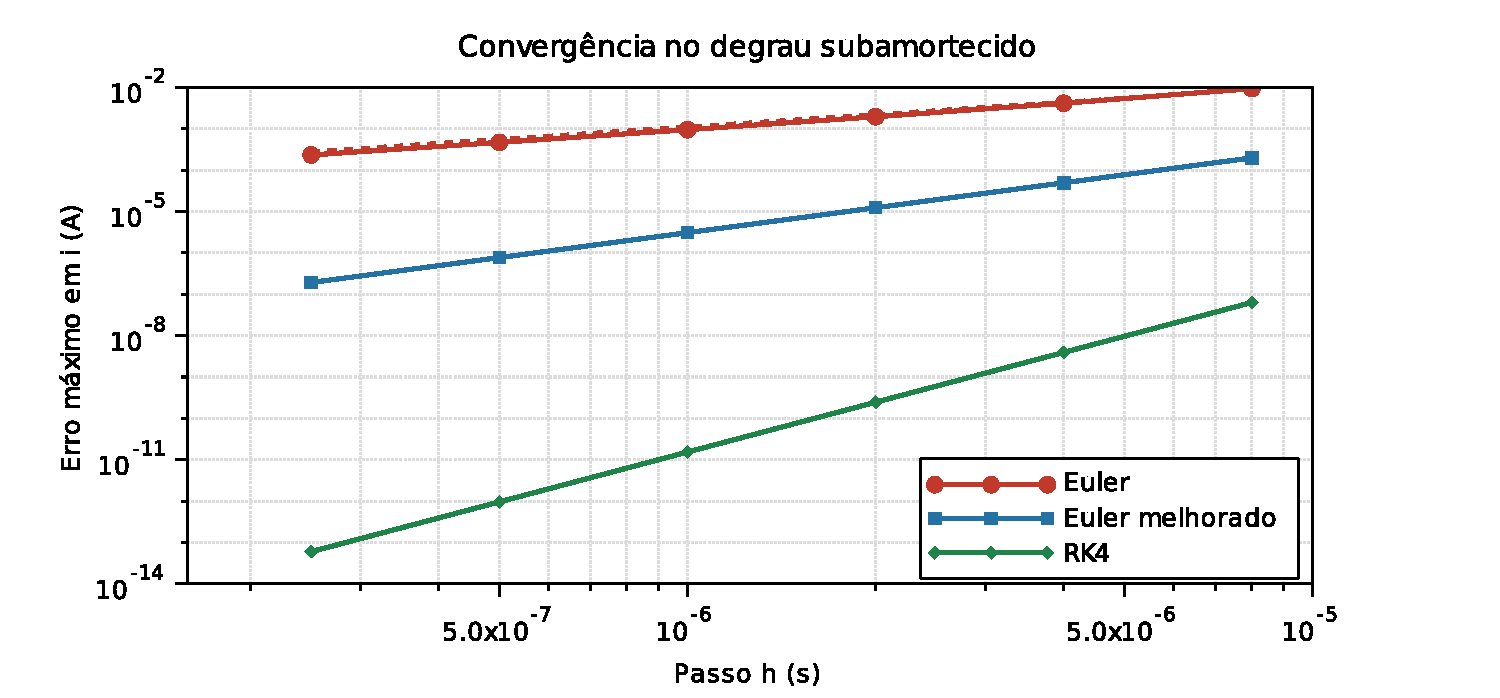
\includegraphics[width=\textwidth]{convergencia.pdf}
\caption{Erro máximo da corrente em função do passo. As retas de referência têm inclinação 1, 2 e 4 e estão ancoradas no maior passo de cada método.}
\label{fig:conv}
\end{figure}

A Figura~\ref{fig:degrau} compara as formas de onda com \(h=15~\mu\mathrm{s}\), ainda estável para o Euler, porém próximo do limite. A solução de Euler oscila por mais tempo do que o circuito: o módulo de \(R(h\lambda)\) é menor do que 1, mas o amortecimento numérico é mais fraco do que \(\alpha\). Heun e RK4 sobrepõem-se à solução analítica nessa escala. A Figura~\ref{fig:erro} separa os três erros. Com \(h=8~\mu\mathrm{s}\), o erro de pico do Euler é da ordem de \(10^{-2}\)~A; o do Heun, de \(10^{-4}\)~A; o do RK4, de \(10^{-8}\)~A. Reduzir o passo a \(2~\mu\mathrm{s}\) divide o erro do Euler por cerca de quatro, o do Heun por cerca de dezesseis e o do RK4 por cerca de duzentos e cinquenta, de novo as potências de \(2^{p}\).

\begin{figure}[htbp]
\centering
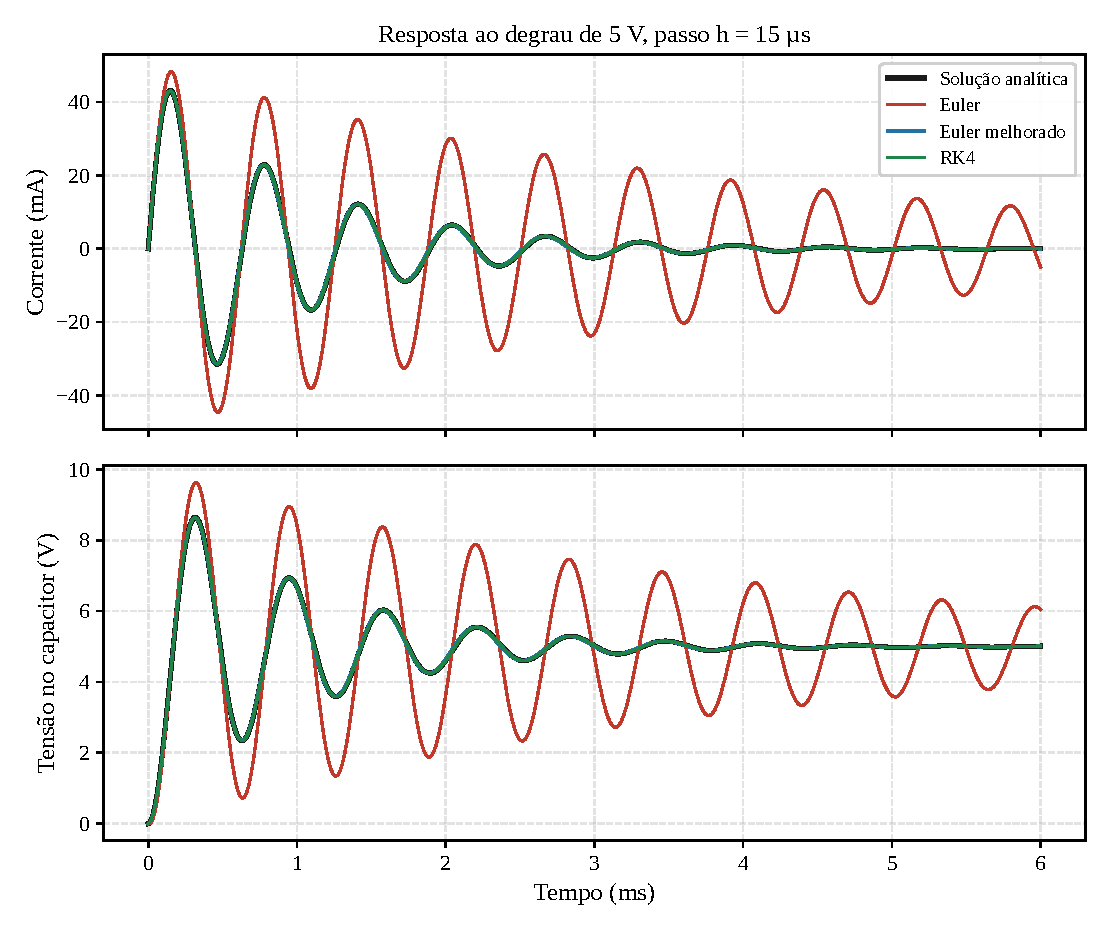
\includegraphics[width=\textwidth]{resposta_degrau.pdf}
\caption{Resposta ao degrau de 5~V com \(R=20~\Omega\) e \(h=15~\mu\mathrm{s}\). Euler ainda é estável, mas o amortecimento numérico é visivelmente menor do que o do circuito.}
\label{fig:degrau}
\end{figure}

\begin{figure}[htbp]
\centering
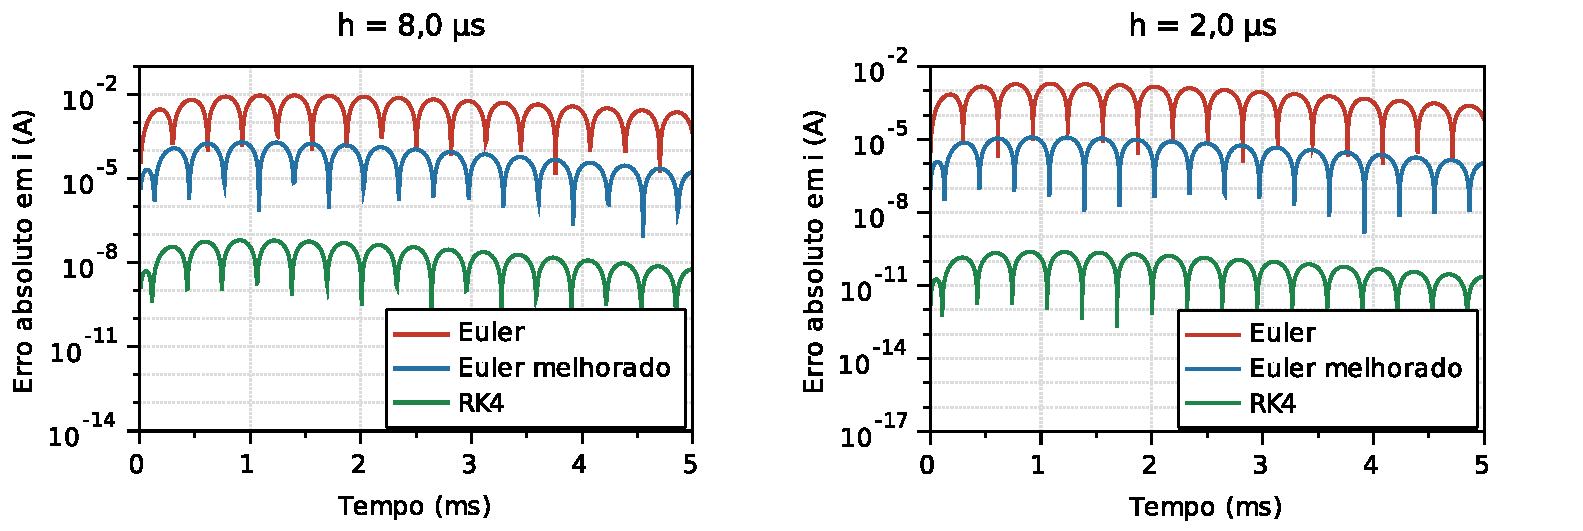
\includegraphics[width=\textwidth]{erro_temporal.pdf}
\caption{Erro absoluto da corrente ao longo do tempo, nos passos de 8~\(\mu\)s e de 2~\(\mu\)s. A oscilação do erro acompanha a corrente do circuito.}
\label{fig:erro}
\end{figure}

\subsection{Regimes de amortecimento}

A Tabela~\ref{tab:regimes} repete os três métodos com \(h=2~\mu\mathrm{s}\) nos três regimes. O RK4 mantém erro máximo de corrente entre \(10^{-10}\) e \(10^{-9}\)~A. O caso sobreamortecido é um pouco pior porque o polo rápido, \(\lambda\approx -4{,}79\times 10^{4}~\mathrm{s}^{-1}\), exige mais do passo: \(h|\lambda|\approx 0{,}096\). Ainda assim, o erro é irrelevante diante de uma corrente de miliampères. A Figura~\ref{fig:regimes} mostra que a curva do RK4 e a curva analítica se confundem nos três regimes. O método não está restrito ao oscilador para o qual a estabilidade é mais delicada.

\begin{table}[htbp]
\centering
\caption{Erro máximo da corrente com \(h=2~\mu\mathrm{s}\) e \(t_f=5~\mathrm{ms}\), nos três regimes.}
\label{tab:regimes}
\small
\begin{tabular}{@{}lrrr@{}}
\toprule
Regime & Euler & Euler melhorado & RK4 \\
\midrule
Subamortecido, \(R=20~\Omega\) & \(1{,}95\times 10^{-3}\) & \(1{,}23\times 10^{-5}\) & \(2{,}46\times 10^{-10}\) \\
Crítico, \(R=200~\Omega\) & \(2{,}34\times 10^{-4}\) & \(2{,}72\times 10^{-6}\) & \(1{,}03\times 10^{-10}\) \\
Sobreamortecido, \(R=500~\Omega\) & \(2{,}00\times 10^{-4}\) & \(6{,}60\times 10^{-6}\) & \(3{,}05\times 10^{-9}\) \\
\bottomrule
\end{tabular}
\end{table}

\begin{figure}[htbp]
\centering
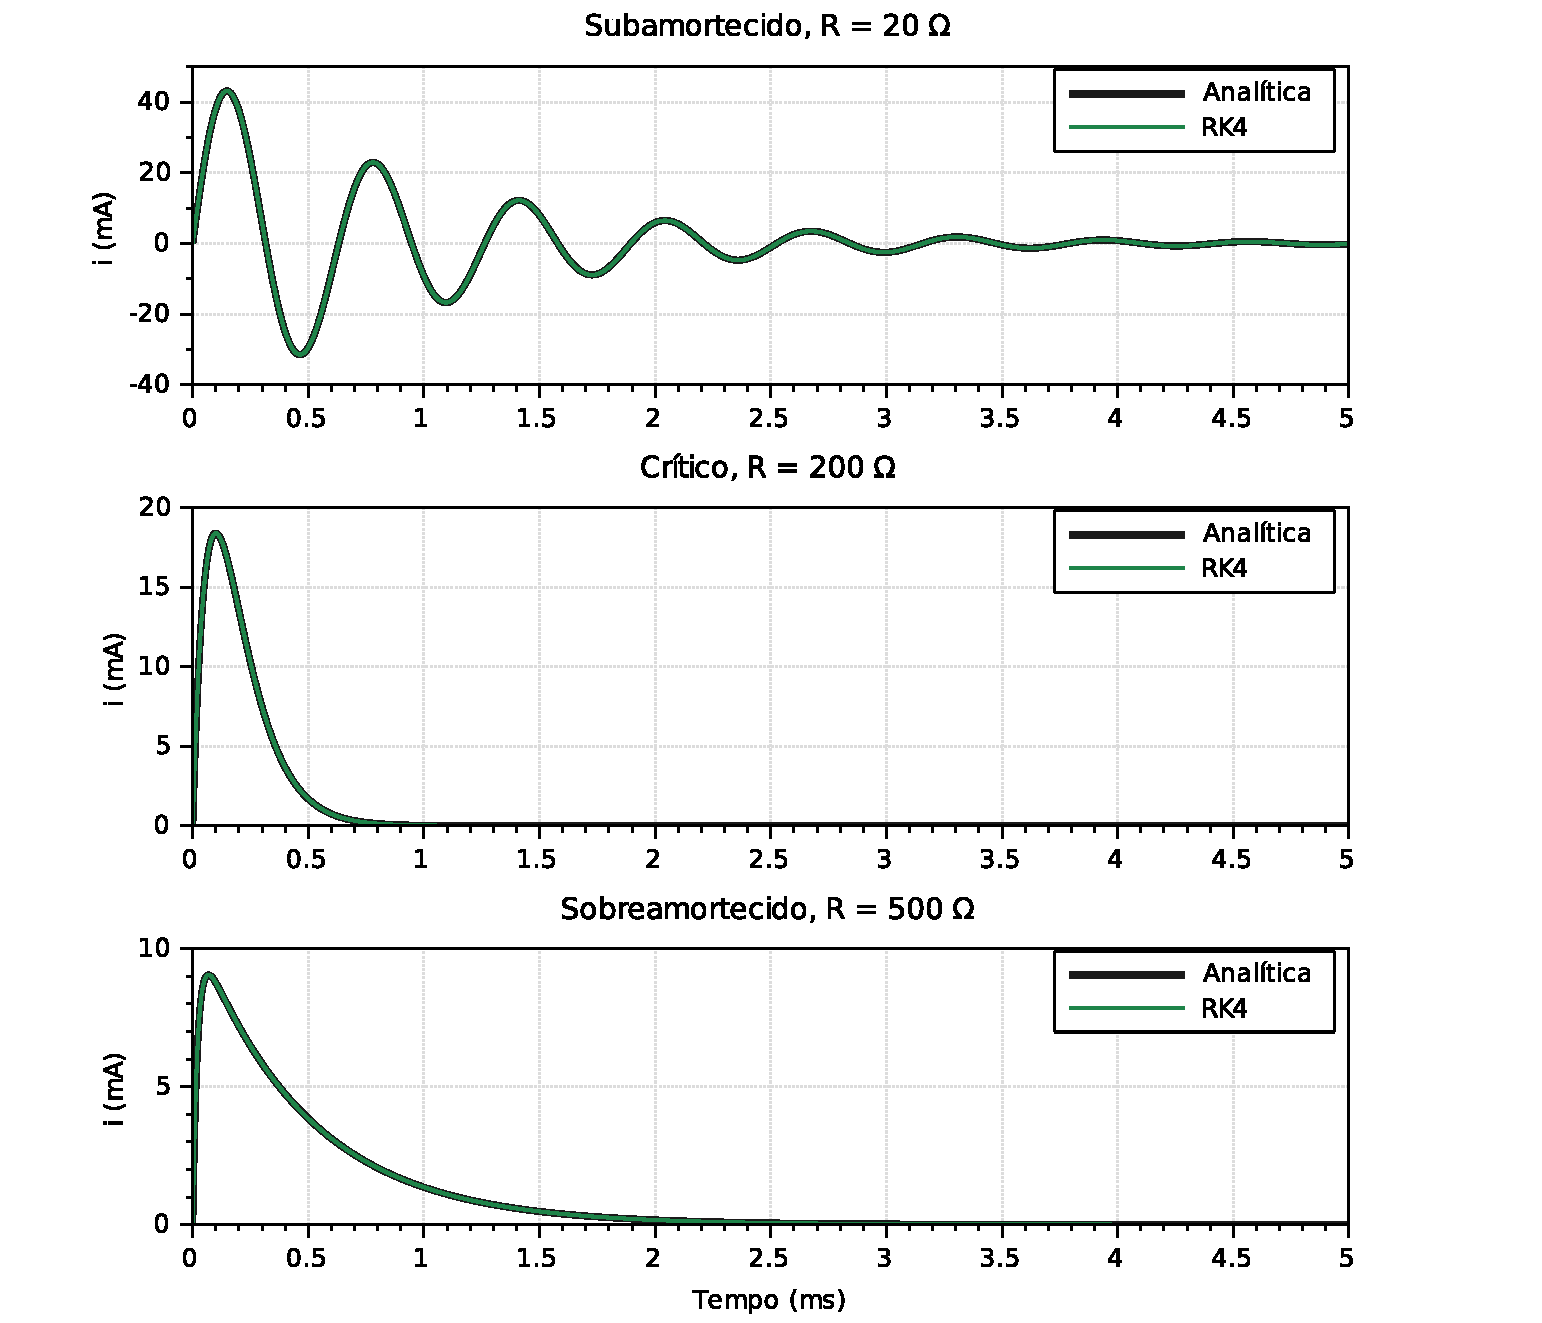
\includegraphics[width=0.94\textwidth]{regimes.pdf}
\caption{Corrente do degrau nos três regimes. A curva analítica e o RK4 com \(h=2~\mu\mathrm{s}\) aparecem sobrepostos.}
\label{fig:regimes}
\end{figure}

\subsection{Estabilidade e fator de qualidade}

A Tabela~\ref{tab:hestab} traz os maiores passos para os quais \(|R(h\lambda)|\le 1\). No Euler subamortecido o valor coincide com \(RC\): 20{,}0~\(\mu\)s para \(Q=5\) e 2{,}00~\(\mu\)s para \(Q=50\). O Heun chega a 104{,}9~\(\mu\)s e a 44{,}4~\(\mu\)s. O RK4 chega a 295{,}0~\(\mu\)s e a 284{,}8~\(\mu\)s. No tanque de alto \(Q\), o limite do RK4 quase não muda, e o do Euler cai dez vezes. O período natural é 628~\(\mu\)s. O Euler com \(Q=50\) precisa de mais de trezentos passos por período só para não divergir. O RK4 ainda é estável com cerca de dois passos por período, embora com erro grande. Estabilidade não é precisão; é a condição para que a precisão possa ser discutida.

\begin{table}[htbp]
\centering
\caption{Maior passo absolutamente estável, obtido da função \(R(z)\) e dos autovalores do circuito.}
\label{tab:hestab}
\small
\begin{tabular}{@{}lrrr@{}}
\toprule
Circuito & Euler & Euler melhorado & RK4 \\
\midrule
\(R=20~\Omega\), \(Q=5\) & 20{,}0~\(\mu\)s & 104{,}9~\(\mu\)s & 295{,}0~\(\mu\)s \\
\(R=2~\Omega\), \(Q=50\) & 2{,}00~\(\mu\)s & 44{,}4~\(\mu\)s & 284{,}8~\(\mu\)s \\
\bottomrule
\end{tabular}
\end{table}

A Figura~\ref{fig:estab} integra o degrau até 6~ms e marca o pico de \(|i|\). As retas verticais são os limites da Tabela~\ref{tab:hestab}. Para \(Q=5\), o pico físico fica perto de 43~mA. Com \(h=25~\mu\mathrm{s}\), o Euler já atinge 0{,}21~A; com \(h=40~\mu\mathrm{s}\), a integração é interrompida pela guarda de divergência. O Heun permanece físico até 80~\(\mu\)s (pico de 45~mA) e chega a 1{,}10~A em 120~\(\mu\)s. O maior passo ensaiado para o RK4 nesse circuito, 286~\(\mu\)s, ainda está abaixo de 295~\(\mu\)s: a solução não explode, mas o pico numérico cai a 30~mA e o erro máximo é 41~mA. O método é estável e, ao mesmo tempo, inútil para ler a amplitude.

Para \(Q=50\), o Euler já cresce em \(h=5~\mu\mathrm{s}\) (pico de 0{,}12~A contra cerca de 49~mA físicos) e atinge 9{,}1~A em 20~\(\mu\)s. O Heun rompe entre 40~\(\mu\)s e 80~\(\mu\)s. O RK4 mantém o pico perto do valor físico até 200~\(\mu\)s e só dá sinal de crescimento no último passo, de 286~\(\mu\)s, ligeiramente acima do limite de 284{,}8~\(\mu\)s. O muro previsto pela função de estabilidade aparece na integração, no lugar previsto.

\begin{figure}[htbp]
\centering
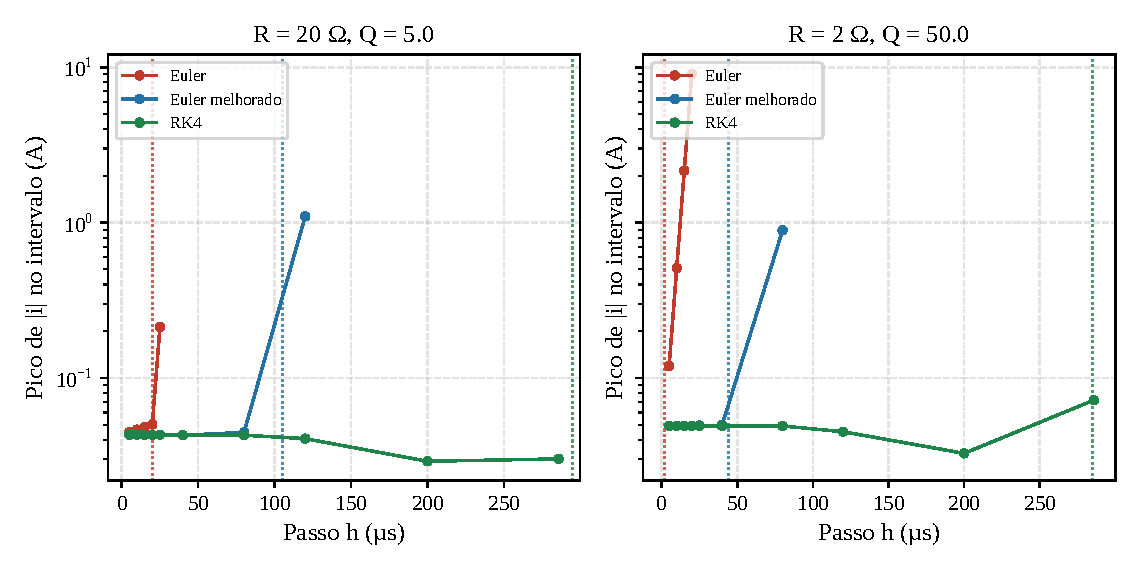
\includegraphics[width=\textwidth]{estabilidade.pdf}
\caption{Pico de \(|i|\) no intervalo de 6~ms, em função do passo. As retas pontilhadas marcam o limite de estabilidade de cada método. Acima dele o pico deixa de ser o pico do circuito.}
\label{fig:estab}
\end{figure}

\subsection{Excitação senoidal}

A Tabela~\ref{tab:seno} usa \(h=1~\mu\mathrm{s}\) e \(t_f=8~\mathrm{ms}\). A amplitude e a fase são as do fasor. O erro indicado é o erro absoluto máximo da corrente ao longo de todo o transitório, não a diferença entre o pico do último período e a amplitude permanente. Essa segunda diferença ainda contém a resposta natural, da ordem de \(e^{-\alpha t_f}\approx 3\times 10^{-4}\) em 8~ms, e não mede o método.

\begin{table}[htbp]
\centering
\caption{Excitação \(5\sin(\omega t)\) com \(R=20~\Omega\) e \(h=1~\mu\mathrm{s}\). A fase usa a senoide como referência.}
\label{tab:seno}
\small
\setlength{\tabcolsep}{4pt}
\begin{tabular}{@{}lrrrrr@{}}
\toprule
Caso & \(|I|\) (mA) & fase & Euler & Heun & RK4 \\
\midrule
\(\omega=\omega_0\) & 250{,}0 & \(0^{\circ}\) & \(1{,}31\times 10^{-2}\) & \(4{,}20\times 10^{-5}\) & \(2{,}09\times 10^{-10}\) \\
\(\omega=0{,}7\,\omega_0\) & 66{,}18 & \(+74{,}6^{\circ}\) & \(1{,}93\times 10^{-3}\) & \(6{,}42\times 10^{-6}\) & \(3{,}11\times 10^{-11}\) \\
\(\omega=1{,}4\,\omega_0\) & 70{,}00 & \(-73{,}7^{\circ}\) & \(2{,}88\times 10^{-3}\) & \(8{,}33\times 10^{-6}\) & \(4{,}58\times 10^{-11}\) \\
\bottomrule
\end{tabular}
\end{table}

Na ressonância a corrente cresce durante alguns milissegundos até 250~mA, como mostra a Figura~\ref{fig:seno}. Fora da ressonância, em \(0{,}7\,\omega_0\), a reatância é capacitiva, a corrente adianta 74{,}6° e a amplitude cai para 66{,}2~mA. Em \(1{,}4\,\omega_0\) a corrente atrasa 73{,}7° e a amplitude é 70{,}0~mA. O RK4 acompanha a forma fechada com erro inferior a \(10^{-9}\)~A. O Euler, no mesmo passo, erra cerca de 13~mA na ressonância, 5\% da amplitude permanente. Para decidir a seletividade de um estágio, esse erro já desloca a leitura.

\begin{figure}[htbp]
\centering
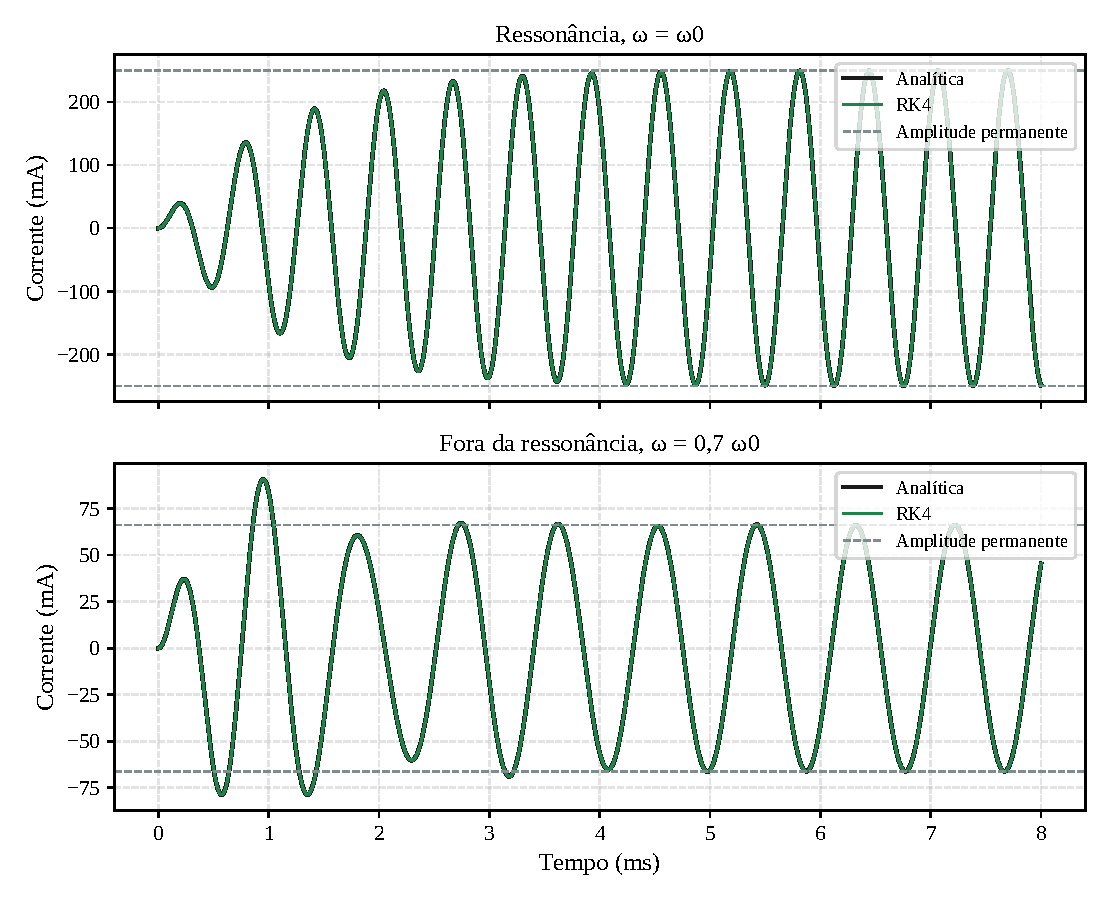
\includegraphics[width=\textwidth]{senoidal.pdf}
\caption{Corrente com excitação senoidal de 5~V e \(h=1~\mu\mathrm{s}\). As retas tracejadas são a amplitude do regime permanente. RK4 e solução analítica se sobrepõem.}
\label{fig:seno}
\end{figure}

\subsection{Custo para um erro prescrito}

Se \(E(h)\approx C h^{p}\) no intervalo em que o truncamento domina, o passo que produz um erro alvo e o número de avaliações em \(T=5~\mathrm{ms}\) seguem de \(h=(E/C)^{1/p}\) e de \(N_f=s\,T/h\), com \(s=1\), 2 ou 4 estágios. A Tabela~\ref{tab:custo} usa o ajuste da Seção~6.1. As metas \(10^{-6}\) e \(10^{-8}\) caem dentro ou na borda da faixa medida para o Heun e para o RK4. A meta \(10^{-6}\) do Euler pede \(h\approx 1{,}5~\mathrm{ns}\), fora da faixa; a extrapolação é aceitável em precisão dupla porque o arredondamento acumulado nesse número de passos, da ordem de \(10^{-11}\)~A, ainda fica abaixo da meta. As metas folgadas de \(10^{-3}\) extrapolam para passos maiores do que 8~\(\mu\)s e devem ser lidas como ordem de grandeza.

\begin{table}[htbp]
\centering
\caption{Avaliações de \(f\) estimadas para um erro máximo de corrente no intervalo de 5~ms.}
\label{tab:custo}
\small
\begin{tabular}{@{}rrrr@{}}
\toprule
Erro alvo (A) & Euler & Euler melhorado & RK4 \\
\midrule
\(10^{-3}\) & \(4{,}87\times 10^{3}\) & \(5{,}55\times 10^{2}\) & \(2{,}23\times 10^{2}\) \\
\(10^{-4}\) & \(4{,}27\times 10^{4}\) & \(1{,}76\times 10^{3}\) & \(3{,}96\times 10^{2}\) \\
\(10^{-6}\) & \(3{,}29\times 10^{6}\) & \(1{,}75\times 10^{4}\) & \(1{,}25\times 10^{3}\) \\
\(10^{-8}\) & \(2{,}54\times 10^{8}\) & \(1{,}75\times 10^{5}\) & \(3{,}96\times 10^{3}\) \\
\bottomrule
\end{tabular}
\end{table}

Para um erro de \(10^{-6}\)~A, o RK4 custa cerca de \(1{,}3\times 10^{3}\) avaliações, o Heun cerca de \(1{,}8\times 10^{4}\) e o Euler cerca de \(3{,}3\times 10^{6}\). Quatro avaliações por passo parecem um sobrecusto quando se olha um único passo. No erro prescrito, o RK4 é o método barato. O Euler só compete se a tolerância for grosseira e o passo couber na região de estabilidade. No circuito de \(Q=50\), essa segunda condição já elimina passos acima de 2~\(\mu\)s, e o custo do Euler sobe antes mesmo da conta da ordem.

\subsection{Passo adaptativo}

No degrau de \(Q=5\), o controlador partiu de \(h=20~\mu\mathrm{s}\). A Tabela~\ref{tab:adap} resume três tolerâncias, com \(\mathrm{atol}=10^{-3}\,\mathrm{rtol}\). O erro global da corrente ficou abaixo da tolerância relativa pedida. O erro da tensão, maior em valor absoluto por causa da escala, corresponde a um erro relativo da ordem da tolerância ou um pouco acima dela, como se espera de um controle local acumulado num intervalo. Cada tentativa custa 12 avaliações, porque há um passo cheio e dois meios passos. Por isso o adaptativo gasta mais avaliações do que um RK4 fixo já sintonizado na mesma precisão: cerca de 2\,400 contra cerca de 1\,300 para um erro de corrente próximo de \(10^{-6}\)~A. Num problema linear de escala fixa, o passo ótimo é quase constante, e o controlador paga a estimativa do erro sem poder economizar passos.

\begin{table}[htbp]
\centering
\caption{RK4 adaptativo no degrau subamortecido, intervalo de 5~ms.}
\label{tab:adap}
\small
\setlength{\tabcolsep}{4pt}
\begin{tabular}{@{}rrrrrr@{}}
\toprule
\(\mathrm{rtol}\) & avaliações & aceitos & rejeitados & erro máx.\ de \(i\) & erro máx.\ de \(v_C\) \\
\midrule
\(10^{-4}\) & 1\,236 & 75 & 28 & \(1{,}65\times 10^{-5}\) & \(1{,}53\times 10^{-3}\) \\
\(10^{-6}\) & 2\,424 & 180 & 22 & \(4{,}62\times 10^{-7}\) & \(4{,}38\times 10^{-5}\) \\
\(10^{-8}\) & 5\,640 & 452 & 18 & \(1{,}11\times 10^{-8}\) & \(1{,}07\times 10^{-6}\) \\
\bottomrule
\end{tabular}
\end{table}

O pulso gaussiano é o caso em que o passo deve variar. A referência fina, com \(h=0{,}25~\mu\mathrm{s}\), consome 64\,000 avaliações. Duas malhas finas, de 0{,}25~\(\mu\)s e 0{,}50~\(\mu\)s, concordam em \(3{,}40\times 10^{-7}\)~A, abaixo do erro do método adaptativo, de modo que a referência segura a comparação. Com \(\mathrm{rtol}=10^{-6}\) e \(\mathrm{atol}=10^{-8}\), o controlador usou 2\,040 avaliações, 149 passos aceitos e 21 rejeitados. O passo chegou a 400~\(\mu\)s enquanto o circuito ainda estava em repouso, caiu para cerca de 8~\(\mu\)s na chegada do pulso e ficou entre 15~\(\mu\)s e 30~\(\mu\)s durante o toque, como mostra a Figura~\ref{fig:pulso}. O erro máximo da corrente foi \(3{,}20\times 10^{-4}\)~A, cerca de 0{,}9\% do pico de 34{,}4~mA. Um passo fixo com o mesmo número de passos aceitos, \(h=26{,}8~\mu\mathrm{s}\), produziu erro de \(9{,}51\times 10^{-4}\)~A. O adaptativo acerta o passo onde a fonte muda e evita o custo da malha fina uniforme. A tolerância local de \(10^{-6}\) não se transferiu automaticamente para um erro global de \(10^{-6}\): o erro realizado é da ordem de \(10^{-4}\)~A. Quem precisar de mais do que isso pede uma tolerância mais apertada, ou limita o passo máximo à região de estabilidade.

\begin{figure}[htbp]
\centering
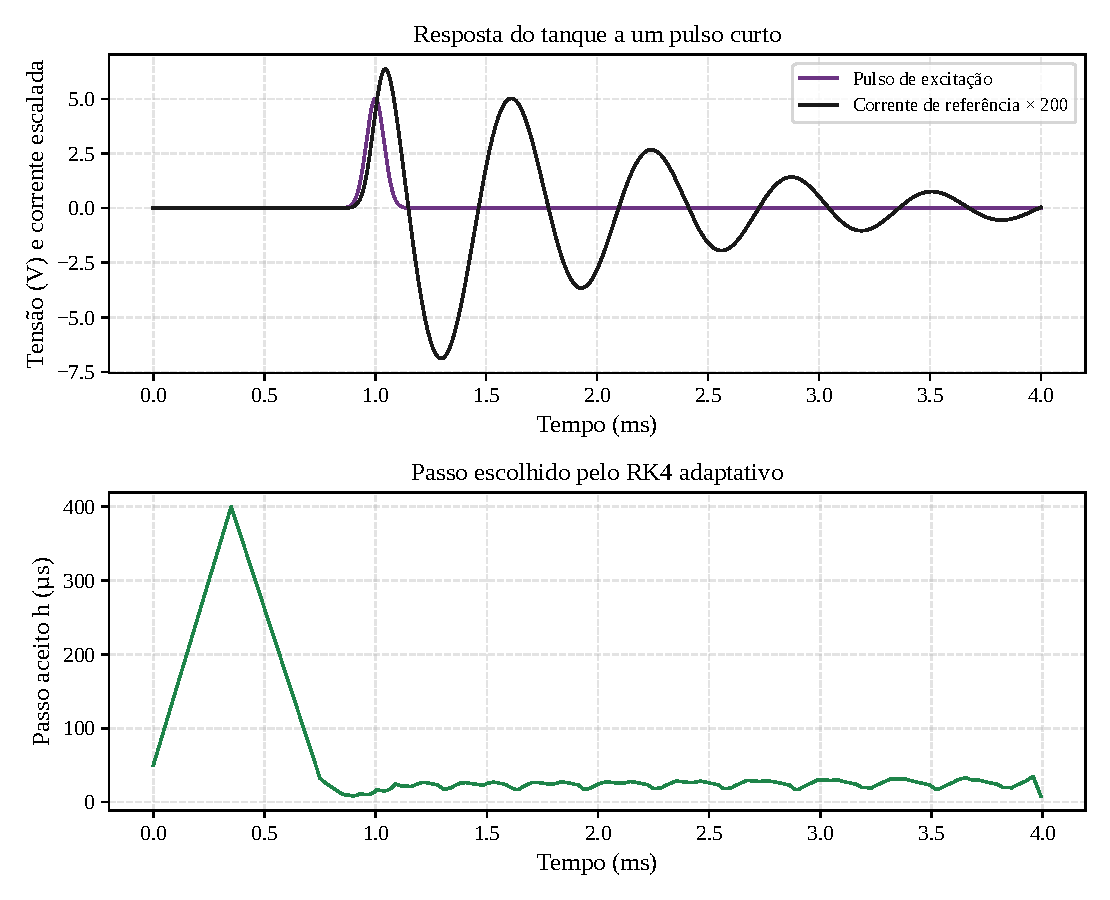
\includegraphics[width=\textwidth]{pulso.pdf}
\caption{Pulso gaussiano de 5~V e passo escolhido pelo RK4 adaptativo. A corrente de referência está multiplicada por 200 para compartilhar o eixo com a tensão da fonte.}
\label{fig:pulso}
\end{figure}

\subsection{Precisão simples e precisão dupla}
\label{sec:precisao}

A Figura~\ref{fig:prec} e a Tabela~\ref{tab:prec} repetem o RK4 do degrau, agora até 4~ms, em \emph{binary64} e \emph{binary32}. Enquanto o truncamento domina, as duas curvas coincidem: em \(h=8~\mu\mathrm{s}\) o erro é \(6{,}3\times 10^{-8}\)~A nos dois formatos. A partir de \(h=4~\mu\mathrm{s}\) a precisão simples descola e passa a oscilar entre \(3\times 10^{-8}\) e \(8\times 10^{-8}\)~A. Refinar mais o passo piora o resultado: em \(h=3{,}125\times 10^{-2}~\mu\mathrm{s}\) o erro sobe a \(4{,}35\times 10^{-7}\)~A. A precisão dupla continua a cair com inclinação 4 até \(3{,}08\times 10^{-16}\)~A, em \(h=6{,}25\times 10^{-2}~\mu\mathrm{s}\), e só então dá um passo para cima, para \(7{,}95\times 10^{-16}\)~A. O épsilon de máquina da precisão simples é \(1{,}19\times 10^{-7}\); o da dupla é \(2{,}22\times 10^{-16}\). O piso observado na corrente, cuja amplitude é de poucos centésimos de ampère, fica uma ordem abaixo do épsilon simples e junto do épsilon duplo no extremo do ensaio.

\begin{table}[htbp]
\centering
\caption{Erro máximo da corrente no RK4, em ampères, conforme o formato IEEE 754. Intervalo de 4~ms.}
\label{tab:prec}
\small
\begin{tabular}{@{}rrr@{}}
\toprule
\(h\) (\(\mu\)s) & \emph{binary64} & \emph{binary32} \\
\midrule
8{,}00 & \(6{,}32\times 10^{-8}\) & \(6{,}05\times 10^{-8}\) \\
4{,}00 & \(3{,}94\times 10^{-9}\) & \(2{,}82\times 10^{-8}\) \\
2{,}00 & \(2{,}46\times 10^{-10}\) & \(6{,}37\times 10^{-8}\) \\
1{,}00 & \(1{,}53\times 10^{-11}\) & \(4{,}07\times 10^{-8}\) \\
0{,}50 & \(9{,}58\times 10^{-13}\) & \(6{,}45\times 10^{-8}\) \\
0{,}25 & \(6{,}00\times 10^{-14}\) & \(8{,}19\times 10^{-8}\) \\
0{,}125 & \(3{,}76\times 10^{-15}\) & \(1{,}94\times 10^{-7}\) \\
0{,}0625 & \(3{,}08\times 10^{-16}\) & \(2{,}03\times 10^{-7}\) \\
0{,}03125 & \(7{,}95\times 10^{-16}\) & \(4{,}35\times 10^{-7}\) \\
\bottomrule
\end{tabular}
\end{table}

\begin{figure}[htbp]
\centering
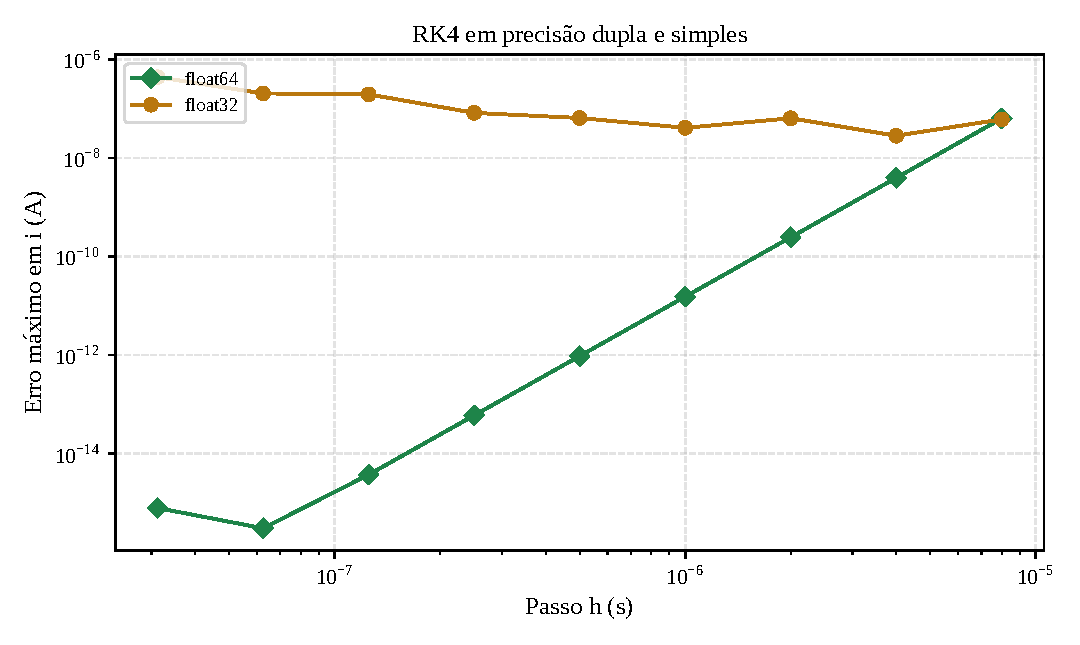
\includegraphics[width=0.92\textwidth]{precisao.pdf}
\caption{Erro do RK4 em precisão dupla e simples. O truncamento cai com o passo; o arredondamento da precisão simples estabelece um piso e, abaixo dele, o erro volta a subir.}
\label{fig:prec}
\end{figure}

O número importa para um processador embarcado ou um DSP que só oferece ponto flutuante de 32 bits em hardware. Neste circuito, gastar um passo menor do que cerca de 1~\(\mu\)s em precisão simples não compra dígito nenhum. Uma corrente de dezenas de miliampères fica com erro absoluto perto de \(10^{-7}\)~A, o que é folgado para desenhar a forma de onda e pode ser curto para uma integração muito longa, para uma diferença de duas simulações próximas ou para um \(Q\) tão alto que a energia dissipada por ciclo seja comparável ao erro acumulado. Precisão dupla emula o formato largo em software, com custo de tempo. O ensaio quantifica o que se troca.

\subsection{Limitações e melhorias}

Os métodos explícitos deste estudo são adequados ao RLC de um único par de polos, com \(Q\) moderado ou alto, desde que o passo respeite a Tabela~\ref{tab:hestab}. Eles deixam de ser a ferramenta certa em três situações. A primeira é o sistema rígido: um circuito com parasitário muito rápido e estado lento força \(h\) pelo polo que não interessa. A segunda é o sistema diferencial-algébrico da análise nodal de uma rede grande, para o qual os métodos implícitos do SPICE foram desenhados. A terceira é a portadora de radiofrequência integrada em tempo absoluto durante muitos símbolos; o caminho econômico é mudar o modelo, não o passo.

Melhorias diretas, sem trocar de família, são um par embarcado com estimativa de erro mais barata do que a duplicação, como Dormand-Prince 5(4), um teto de passo igual ao limite de estabilidade linear e soma compensada para adiar o piso de arredondamento. Um método implícito, ainda que apenas a regra trapezoidal, seria o experimento natural de continuação: a mesma equação, a mesma referência analítica e uma região de estabilidade que cobre o semieixo real negativo. A comparação isolaria o que, neste trabalho, aparece como muro do método explícito.

\section{Conclusão}
\label{sec:conclusao}

O cálculo numérico chegou aos computadores com os métodos já formulados. Newton, Euler, Lagrange, Gauss, Jacobi, Runge e Kutta produziram procedimentos de aproximação para tabelas, órbitas e equações diferenciais muito antes do ENIAC. Babbage e Lovelace separaram a máquina da sequência de operações. O ponto flutuante, padronizado pelo IEEE 754 e já presente nas máquinas de Zuse, fixou o erro que nenhuma ordem de convergência apaga. Linguagens como Fortran, MATLAB, Scilab, Python e Julia, e bibliotecas como BLAS e LAPACK, transformaram esses procedimentos em ferramenta diária de engenharia.

No problema escolhido, essa história aparece como número. O Euler, o Euler melhorado e o RK4 clássico, implementados sem integrador de biblioteca, reproduziram as ordens 1, 2 e 4 na resposta ao degrau de um RLC série. O limite de estabilidade do Euler é \(RC\), ou \(1/(\omega_0 Q)\): 20~\(\mu\)s com \(Q=5\) e 2~\(\mu\)s com \(Q=50\). O RK4 permanece estável até cerca de 285~\(\mu\)s no tanque seletivo. Para um erro de \(10^{-6}\)~A em 5~ms, a conta de avaliações favorece o método de quarta ordem por três ordens de grandeza em relação ao Euler. A senoide na ressonância e fora dela, e os regimes crítico e sobreamortecido, confirmam que o erro medido contra a forma fechada acompanha essa previsão. O controlador adaptativo economiza trabalho quando a fonte tem um trecho morto e um pulso, e não substitui um passo fixo bem escolhido quando a escala de tempo é constante. Em precisão simples, reduzir o passo abaixo de cerca de 1~\(\mu\)s deixa de melhorar o RK4.

O estudo entrega, portanto, uma implementação verificada, uma região de uso e uma região em que o resultado numérico deixa de ser o circuito. A continuação natural é a regra trapezoidal no mesmo RLC, um par adaptativo de custo menor e a formulação em envoltória para o estágio de radiofrequência cujo protótipo foi integrado aqui em banda baixa.

\section*{Nota sobre o uso de inteligência artificial}
\addcontentsline{toc}{section}{Nota sobre o uso de inteligência artificial}

Este trabalho declara o uso da ferramenta de inteligência artificial Grok, da xAI, no ambiente Grok Build, como apoio à organização do texto, à redação técnica e ao desenvolvimento e à depuração do código. Os resultados numéricos foram produzidos pela execução do programa do Apêndice~\ref{ap:codigo} e conferidos contra as soluções analíticas derivadas no texto. O uso da ferramenta fica registrado para cumprimento da regra da disciplina. O autor é responsável pelo conteúdo e pela compreensão dos métodos e do código.

\begin{thebibliography}{99}
\addcontentsline{toc}{section}{Referências}

\bibitem[ANDERSON et al.(1999)]{anderson1999}
ANDERSON, E. et al. \textbf{LAPACK users' guide}. 3. ed. Philadelphia: SIAM, 1999.

\bibitem[BACKUS(1979)]{backus1979}
BACKUS, John. The history of FORTRAN I, II, and III. \textbf{IEEE Annals of the History of Computing}, v. 1, n. 1, p. 21--37, 1979.

\bibitem[BEZANSON et al.(2017)]{bezanson2017}
BEZANSON, Jeff; EDELMAN, Alan; KARPINSKI, Stefan; SHAH, Viral B. Julia: a fresh approach to numerical computing. \textbf{SIAM Review}, v. 59, n. 1, p. 65--98, 2017.

\bibitem[BOYCE; DIPRIMA(2012)]{boyce2012}
BOYCE, William E.; DIPRIMA, Richard C. \textbf{Elementary differential equations and boundary value problems}. 10. ed. Hoboken: Wiley, 2012.

\bibitem[BURDEN; FAIRES; BURDEN(2016)]{burden2016}
BURDEN, Richard L.; FAIRES, J. Douglas; BURDEN, Annette M. \textbf{Numerical analysis}. 10. ed. Boston: Cengage Learning, 2016.

\bibitem[BUTCHER(2016)]{butcher2016}
BUTCHER, John C. \textbf{Numerical methods for ordinary differential equations}. 3. ed. Chichester: John Wiley \& Sons, 2016.

\bibitem[BUTCHER; WANNER(1996)]{butcher1996}
BUTCHER, John C.; WANNER, Gerhard. Runge-Kutta methods: some historical notes. \textbf{Applied Numerical Mathematics}, v. 22, n. 1--3, p. 113--151, 1996.

\bibitem[CHAPRA; CANALE(2015)]{chapra2015}
CHAPRA, Steven C.; CANALE, Raymond P. \textbf{Numerical methods for engineers}. 7. ed. New York: McGraw-Hill Education, 2015.

\bibitem[COMPUTER HISTORY MUSEUM(s.d.)]{chm}
COMPUTER HISTORY MUSEUM. \textbf{A key component: the operational amplifier}. Mountain View. Disponível em: \url{https://www.computerhistory.org/revolution/analog-computers/3/154}. Acesso em: 23 nov. 2026.

\bibitem[EULER(1768)]{euler1768}
EULER, Leonhard. \textbf{Institutionum calculi integralis}. Petropolis: Academia Imperialis Scientiarum, 1768. v. 1.

\bibitem[FRANCO(2006)]{franco2006}
FRANCO, Neide Bertoldi. \textbf{Cálculo numérico}. São Paulo: Pearson Prentice Hall, 2006.

\bibitem[FRIGO; JOHNSON(2005)]{frigo2005}
FRIGO, Matteo; JOHNSON, Steven G. The design and implementation of FFTW3. \textbf{Proceedings of the IEEE}, v. 93, n. 2, p. 216--231, 2005.

\bibitem[GOLDBERG(1991)]{goldberg1991}
GOLDBERG, David. What every computer scientist should know about floating-point arithmetic. \textbf{ACM Computing Surveys}, v. 23, n. 1, p. 5--48, 1991.

\bibitem[GOLDSTINE(1972)]{goldstine1972}
GOLDSTINE, Herman H. \textbf{The computer from Pascal to von Neumann}. Princeton: Princeton University Press, 1972.

\bibitem[GOMEZ(1999)]{gomez1999}
GOMEZ, Claude (ed.). \textbf{Engineering and scientific computing with Scilab}. Boston: Birkhäuser, 1999.

\bibitem[HAIRER; NØRSETT; WANNER(1993)]{hairer1993}
HAIRER, Ernst; NØRSETT, Syvert P.; WANNER, Gerhard. \textbf{Solving ordinary differential equations I: nonstiff problems}. 2. ed. Berlin: Springer, 1993.

\bibitem[HARRIS et al.(2020)]{harris2020}
HARRIS, Charles R. et al. Array programming with NumPy. \textbf{Nature}, v. 585, p. 357--362, 2020.

\bibitem[HEUN(1900)]{heun1900}
HEUN, Karl. Neue Methode zur approximativen Integration der Differentialgleichungen einer unabhängigen Veränderlichen. \textbf{Zeitschrift für Mathematik und Physik}, v. 45, p. 23--38, 1900.

\bibitem[HIGHAM(2002)]{higham2002}
HIGHAM, Nicholas J. \textbf{Accuracy and stability of numerical algorithms}. 2. ed. Philadelphia: SIAM, 2002.

\bibitem[HOPP(1999)]{hopp1999}
HOPP, Peter M. \textbf{Slide rules: their history, models and makers}. Mendham: Astragal Press, 1999.

\bibitem[IEEE(2019)]{ieee2019}
IEEE. \textbf{IEEE Std 754-2019}: IEEE standard for floating-point arithmetic. New York: IEEE, 2019.

\bibitem[JUNG(2005)]{jung2005}
JUNG, Walter G. (ed.). \textbf{Op amp applications handbook}. Burlington: Newnes, 2005.

\bibitem[KUTTA(1901)]{kutta1901}
KUTTA, Wilhelm. Beitrag zur näherungsweisen Integration totaler Differentialgleichungen. \textbf{Zeitschrift für Mathematik und Physik}, v. 46, p. 435--453, 1901.

\bibitem[LATHI; DING(2009)]{lathi2009}
LATHI, B. P.; DING, Zhi. \textbf{Modern digital and analog communication systems}. 4. ed. New York: Oxford University Press, 2009.

\bibitem[LAWSON; HANSON; KINCAID; KROGH(1979)]{lawson1979}
LAWSON, Charles L.; HANSON, Richard J.; KINCAID, David R.; KROGH, Fred T. Basic linear algebra subprograms for Fortran usage. \textbf{ACM Transactions on Mathematical Software}, v. 5, n. 3, p. 308--323, 1979.

\bibitem[LEIBNIZ(1703)]{leibniz1703}
LEIBNIZ, Gottfried Wilhelm. Explication de l'arithmétique binaire. \textbf{Mémoires de mathématique et de physique de l'Académie royale des sciences}, Paris, 1703.

\bibitem[LENSTRA; LENSTRA JR.; LOVÁSZ(1982)]{lenstra1982}
LENSTRA, A. K.; LENSTRA JR., H. W.; LOVÁSZ, L. Factoring polynomials with rational coefficients. \textbf{Mathematische Annalen}, v. 261, p. 515--534, 1982.

\bibitem[L'ECUYER(2017)]{lecuyer2017}
L'ECUYER, Pierre. History of uniform random number generation. In: WINTER SIMULATION CONFERENCE, 2017, Las Vegas. \textbf{Proceedings} [...]. Piscataway: IEEE, 2017.

\bibitem[MENABREA(1843)]{menabrea1843}
MENABREA, Luigi Federico. Sketch of the Analytical Engine invented by Charles Babbage. Tradução e notas de Augusta Ada King, Condessa de Lovelace. \textbf{Scientific Memoirs}, Londres, v. 3, p. 666--731, 1843.

\bibitem[MOLER(2004)]{moler2004}
MOLER, Cleve B. \textbf{Numerical computing with MATLAB}. Philadelphia: SIAM, 2004.

\bibitem[NAGEL(1975)]{nagel1975}
NAGEL, Laurence W. \textbf{SPICE2: a computer program to simulate semiconductor circuits}. Berkeley: University of California, Electronics Research Laboratory, 1975. Memorandum n. ERL-M520.

\bibitem[NILSSON; RIEDEL(2019)]{nilsson2019}
NILSSON, James W.; RIEDEL, Susan A. \textbf{Electric circuits}. 11. ed. Boston: Pearson, 2019.

\bibitem[OPPENHEIM; WILLSKY; NAWAB(1997)]{oppenheim1997}
OPPENHEIM, Alan V.; WILLSKY, Alan S.; NAWAB, S. Hamid. \textbf{Signals and systems}. 2. ed. Upper Saddle River: Prentice Hall, 1997.

\bibitem[OVERTON(2001)]{overton2001}
OVERTON, Michael L. \textbf{Numerical computing with IEEE floating point arithmetic}. Philadelphia: SIAM, 2001.

\bibitem[PRESS; TEUKOLSKY; VETTERLING; FLANNERY(2007)]{press2007}
PRESS, William H.; TEUKOLSKY, Saul A.; VETTERLING, William T.; FLANNERY, Brian P. \textbf{Numerical recipes: the art of scientific computing}. 3. ed. Cambridge: Cambridge University Press, 2007.

\bibitem[QUARTERONI; SACCO; SALERI(2007)]{quarteroni2007}
QUARTERONI, Alfio; SACCO, Riccardo; SALERI, Fausto. \textbf{Numerical mathematics}. 2. ed. Berlin: Springer, 2007.

\bibitem[RAND CORPORATION(1955)]{rand1955}
RAND CORPORATION. \textbf{A million random digits with 100,000 normal deviates}. Glencoe: Free Press, 1955.

\bibitem[ROJAS(1997)]{rojas1997}
ROJAS, Raúl. Konrad Zuse's legacy: the architecture of the Z1 and Z3. \textbf{IEEE Annals of the History of Computing}, v. 19, n. 2, p. 5--16, 1997.

\bibitem[RUGGIERO; LOPES(1996)]{ruggiero1996}
RUGGIERO, Márcia A. Gomes; LOPES, Vera Lúcia da Rocha. \textbf{Cálculo numérico: aspectos teóricos e computacionais}. 2. ed. São Paulo: Makron Books, 1996.

\bibitem[RUNGE(1895)]{runge1895}
RUNGE, Carl. Über die numerische Auflösung von Differentialgleichungen. \textbf{Mathematische Annalen}, v. 46, p. 167--178, 1895.

\bibitem[SCILAB(2013)]{scilab2013}
SCILAB. \textbf{History}. 2013. Disponível em: \href{https://web.archive.org/web/20130317145202/http://www.scilab.org/scilab/history}{\nolinkurl{https://web.archive.org/web/20130317145202/}\penalty-10000 \nolinkurl{http://www.scilab.org/scilab/history}}. Acesso em: 23 nov. 2026.

\bibitem[SWADE(2001)]{swade2001}
SWADE, Doron. \textbf{The difference engine: Charles Babbage and the quest to build the first computer}. New York: Viking, 2001.

\bibitem[VIRTANEN et al.(2020)]{virtanen2020}
VIRTANEN, Pauli et al. SciPy 1.0: fundamental algorithms for scientific computing in Python. \textbf{Nature Methods}, v. 17, p. 261--272, 2020.

\bibitem[VON NEUMANN(1945)]{vonneumann1945}
VON NEUMANN, John. \textbf{First draft of a report on the EDVAC}. Philadelphia: Moore School of Electrical Engineering, University of Pennsylvania, 1945.

\bibitem[WILLIAMS(1997)]{williams1997}
WILLIAMS, Michael R. \textbf{A history of computing technology}. 2. ed. Los Alamitos: IEEE Computer Society Press, 1997.

\end{thebibliography}

\appendix
\section{Código-fonte da implementação}
\label{ap:codigo}

O código abaixo é o programa executado para produzir as tabelas e as figuras do trabalho. O espaçamento do apêndice é simples para que a listagem permaneça legível; o corpo do trabalho usa espaçamento 1,5. A linguagem é Python 3. Os métodos de Euler, de Euler melhorado, de Runge-Kutta de quarta ordem e o controlador de passo estão implementados nas funções \texttt{passo\_euler}, \texttt{passo\_heun}, \texttt{passo\_rk4} e \texttt{rk4\_adaptativo}.

\begin{singlespace}
\VerbatimInput[%
  fontsize=\footnotesize,%
  numbers=left,%
  numbersep=6pt,%
  breaklines=true,%
  breakanywhere=true%
]{codigo/rlc_runge_kutta.py}
\end{singlespace}

\end{document}
